\documentclass[conference]{IEEEtran}
\usepackage{arydshln}
\usepackage{booktabs} % For formal tables
\usepackage{minted}
\usepackage{graphicx}
\usepackage{arydshln}
\usepackage{subcaption}
\usepackage{times}
\usepackage{hyperref}
\hypersetup{
    colorlinks=true,
    linkcolor=blue,
    filecolor=magenta,      
    urlcolor=cyan,
}
\usepackage[noadjust]{cite}



% save space
\setlength{\belowcaptionskip}{-2pt}


\begin{document}
\title{Programmable Caches with a Data Management Language \& Policy Engine}
%\titlenote{Produces the permission block, and
%  copyright information}
%\subtitle{Extended Abstract}
%\subtitlenote{The full version of the author's guide is available as
%  \texttt{acmart.pdf} document}
%`
\author{
\IEEEauthorblockN{Michael A. Sevilla, Carlos Maltzahn, Peter Alvaro, *Bradley W. Settlemyer}
\IEEEauthorblockN{*Danny Perez, *David Rich, *Galen M. Shipman}
\IEEEauthorblockN{University of California, Santa Cruz, *Los Alamos National Laboratory}
\IEEEauthorblockN{msevilla@soe.ucsc.edu, \{carlosm, palvaro\}@ucsc.edu, \{bws, danny\_perez, dor, gshipman\}@lanl.gov}}
%
% The code below should be generated by the tool at
% http://dl.acm.org/ccs.cfm
% Please copy and paste the code instead of the example below. 
%
%\begin{CCSXML}
%<ccs2012>
% <concept>
%  <concept_id>10010520.10010553.10010562</concept_id>
%  <concept_desc>Computer systems organization~Embedded systems</concept_desc>
%  <concept_significance>500</concept_significance>
% </concept>
% <concept>
%  <concept_id>10010520.10010575.10010755</concept_id>
%  <concept_desc>Computer systems organization~Redundancy</concept_desc>
%  <concept_significance>300</concept_significance>
% </concept>
% <concept>
%  <concept_id>10010520.10010553.10010554</concept_id>
%  <concept_desc>Computer systems organization~Robotics</concept_desc>
%  <concept_significance>100</concept_significance>
% </concept>
% <concept>
%  <concept_id>10003033.10003083.10003095</concept_id>
%  <concept_desc>Networks~Network reliability</concept_desc>
%  <concept_significance>100</concept_significance>
% </concept>
%</ccs2012>  
%\end{CCSXML}

%\ccsdesc[500]{Computer systems organization~Embedded systems}
%\ccsdesc[300]{Computer systems organization~Redundancy}
%\ccsdesc{Computer systems organization~Robotics}
%\ccsdesc[100]{Networks~Network reliability}
%
%
%\keywords{ACM proceedings, \LaTeX, text tagging}


\maketitle

%\section{Motivation}

The PDSW about ParSplice~\cite{perez:jctc20150parsplice} shows:
\begin{enumerate}
  \item keyspace is structured
  \item we don't need an unlimited cache
  \item dynamic policy works for a while
\end{enumerate}

The machine learning portion classifies read throughput into regimes. We could
like the machine learning to detect the superbasins.

\section{Keyspace Locality}


\section{Machine Learning Techniques}
\begin{itemize}
  \item K-means
  \item DBScane
  \item online learning
\end{itemize}

\section{Implementation}
\begin{itemize}
  \item HXHIM
\end{itemize}

\begin{abstract}

Our analysis of the key-value activity generated by the ParSplice molecular
dynamics simulation demonstrates the need for more complex cache management
strategies. Baseline measurements show clear key access patterns and hot spots
that offer significant opportunity for optimization. We use the data management
language and policy engine from the Mantle system to dynamically explore a
variety of techniques, ranging from basic algorithms and heuristics to
statistical models, calculus, and machine learning. While Mantle was originally
designed for distributed file systems, we show how the collection of
abstractions effectively decomposes the problem into manageable policies for a
different application and storage system.  Our exploration of this space results in a
dynamically sized cache policy that sacrifices negligible performance while
using 32-66\% less memory than the default ParSplice configuration.

\end{abstract}

\section{Introduction}

Storage systems use software-based caches to improve performance but the
policies that guide what data to evict and when to evict vary with the use
case. For example, caching file system metadata on clients and servers reduces
the number of remote procedure calls and improves the performance of
create-heavy workloads common in HPC~\cite{ren:sc2014-indexfs,
patil:fast2011-giga+}. But the policies for what data to evict and when to
evict are specific to the application's behavior and the system's configuration
(hardware, settings, etc.) so a new workload may prove to be a poor match for
the selected caching
policy~\cite{xiao:socc15-shardfs,brandt:msst2003-lh,sevilla:sc15-mantle,
weil:sc2004-dyn-metadata, weil:osdi2006-ceph}. In this paper, we evaluate a
variety of caching policies using our data management language/policy engine and
arrive at a customized policy that works well for our target application.  This
process of trying general policies and quickly iterating to a customized
solution shows that our prototype can be adapted to different workloads.

Our example application, ParSplice~\cite{perez:jctc20150parsplice}, is
representative of an important class applications with similar working set
behaviors that extensively use software-based caches.  ParSplice is a molecular
dynamics simulation that uses a hierarchy of caches and a single persistent
key-value store to store both observed minima across a molecule's equation of
motion (EOM) and the hundreds or thousands of partial trajectories calculated
each second during a parallel job.  This workload is pervasive across
simulations that rely on a mesh-based decomposition of a physical region and
result in millions or billions of mesh cells, where each cell contains
materials, pressures, temperatures and other characteristics that are required
to accurately simulate phenomena of interest.  The fine-grained data annotation
capabilities provided by key-value storage is a natural match for these types
of scientific simulations.  Unfortunately, simulations of this size saturate
the capacity and bandwidth capabilities of a single node so we need more
effective data management techniques.

\begin{figure}[t]
\noindent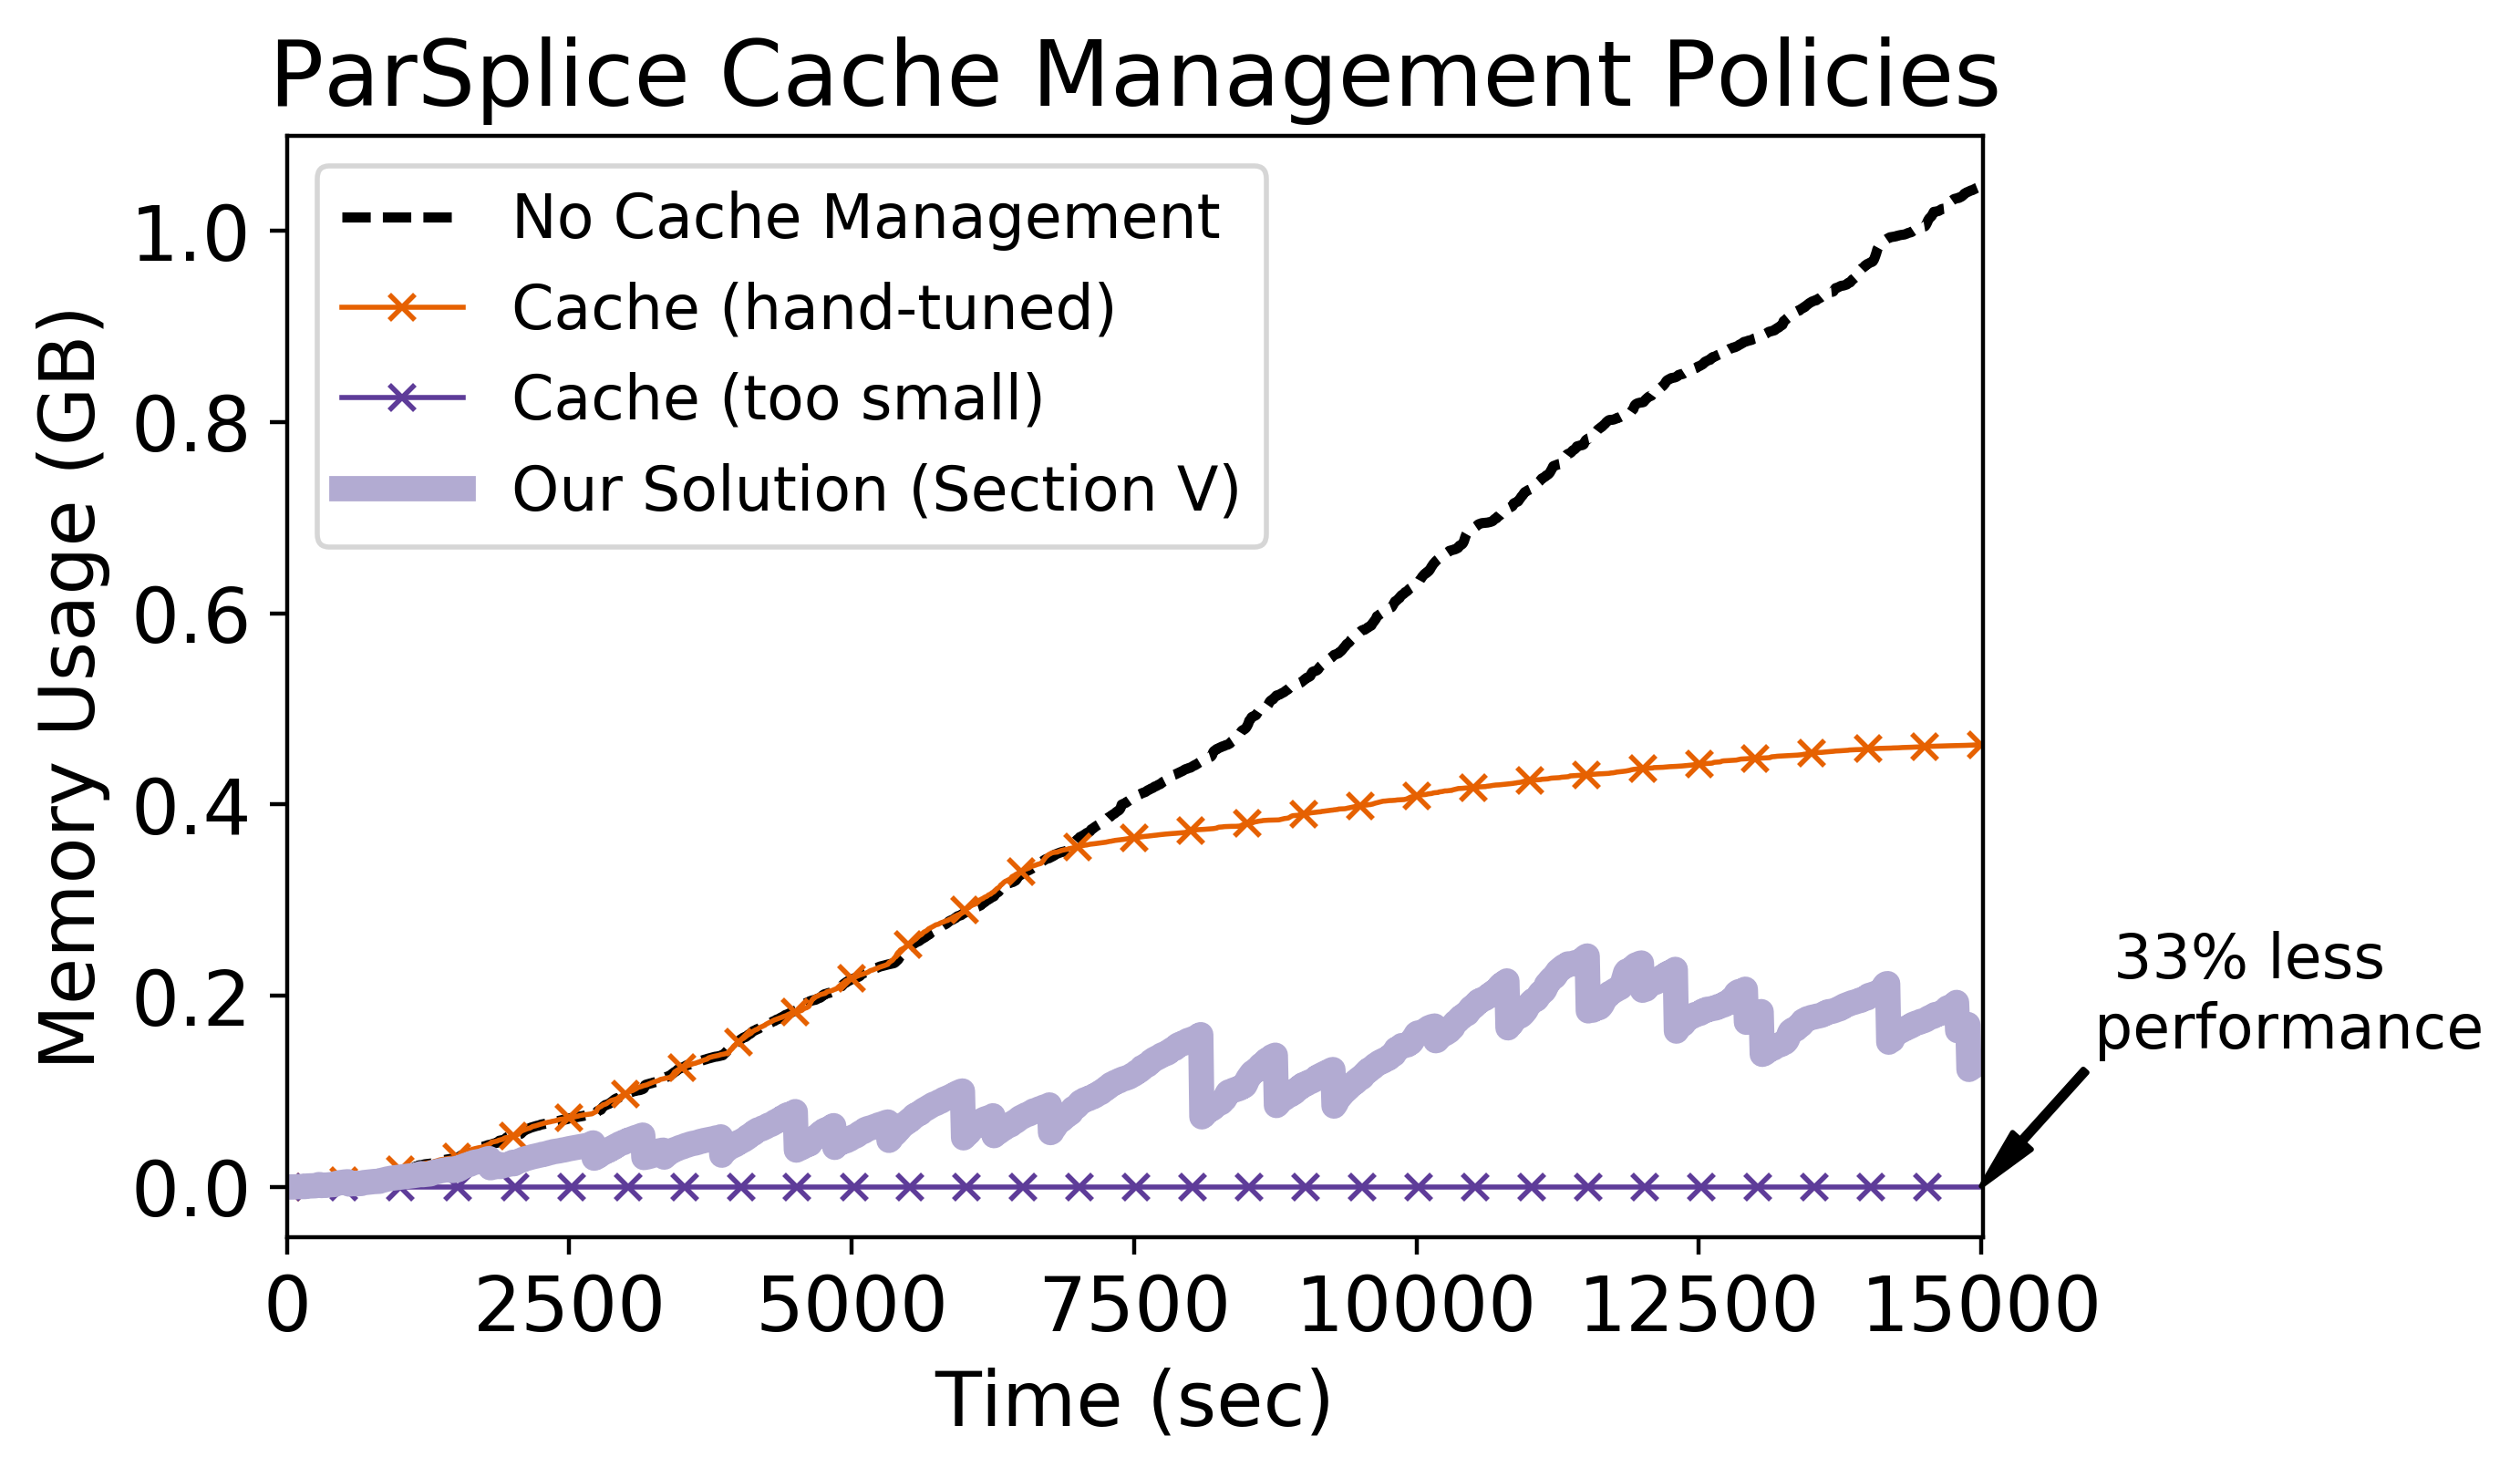
\includegraphics[width=0.5\textwidth]{figures/cache-management.png}\\
\caption{Using our data management language and policy engine, we design a
dynamically sized caching policy (thick line) for ParSplice.  Compared to
existing configurations (thin lines with \(\times\)'s), our solution saves the most
memory without sacrificing performance and works for a variety of inputs.
\label{fig:cache-management}}
\end{figure}

The biggest challenge for ParSplice is properly sizing the caches in the
storage hierarchy.  The memory usage for a single cache that stores molecule
coordinates is shown in Figure~\ref{fig:cache-management}, where the thin solid
lines marked with \(\times\)'s are the existing configurations in ParSplice.
The default configuration uses an unlimited sized cache, shown by the ``No
Cache Management" line, but using this much memory for one cache is
unacceptable for HPC environments, where a common goal is to keep memory for
such data structures below 3\%\footnote{Anecdotally, we find this threshold
works well for HPC applications.  For reference, a 1GB cache for a distributed
file system is too large in LANL deployments.}. Furthermore, ParSplice deploys
a cache per 300 worker processes, so large simulations need more caches and
will use even more memory.  Users can configure ParSplice to evict data when
the cache reaches a threshold but this solution requires tuning and parameter
sweeps; the ``Cache (too small)" curve in Figure~\ref{fig:cache-management}
shows how a poorly configured cache can save memory but at the cost of
performance, which is shown by the text annotation to the right.  Even worse,
this threshold changes with different initial configurations and cluster setups
so tuning needs to be done for all system permutations.  Our dynamically sized
cache, shown by the thick line in Figure~\ref{fig:cache-management}, detects
key access patterns and re-sizes the cache accordingly.  Without tuning or
parameter sweeps, our solution saves more memory than a hand-tuned cache with a
negligible performance degradation (within the baseline's standard deviation),
works for a variety of initial conditions, and could generalize to similar
applications.

% What is Mantle
To design more flexible cache management policies, like our solution in
Figure~\ref{fig:cache-management}, we use the data management language and
policy engine from the Mantle paper~\cite{sevilla:sc15-mantle}.  While Mantle
was designed for the narrow purpose of file system metadata load balancing,
this paper provides evidence that the approach is more broad.  Specifically,
the collection of abstractions in Mantle provide a general control plane that
improves the performance of metadata access. So in this paper we refer to
Mantle as a policy engine that injects policies written in our data management
language directly into a running storage system, such as a file system or key-value
store.  Rather than implementing a policy directly into the storage system,
which requires domain-specific knowledge to find and change policies in the
storage system, we separate policies from mechanisms in a general way.  By
exposing just the policies developers unfamiliar with the storage system that
their application uses can quickly deploy efficient solutions based on their
application-specific knowledge.  We show that our framework:

\begin{itemize}

  \item decomposes cache management into independent policies that can be
  dynamically changed, making the problem more manageable and easier to reason
  about.

  \item can deploy a variety of cache management strategies ranging from basic
  algorithms and heuristics to statistical models and machine learning.

  \item has useful primitives that, while designed for file system metadata
  load balancing, turn out to also be effective for cache management. 

\end{itemize}

% this gives us many policies that are effective across disciplines
% - reuse: eases burden of writing policies
% - autonomic: lays groundwork for an adaptable policy that mixes/matches policies
% FUTURE WORK

This last contribution is explored in Sections~\S\ref{sec:arch-specific}
and~\S\ref{sec:dom-specific}, where we try a range of policies from different
disciplines; but more importantly, in Section~\S\ref{sec:scope}, we conclude
that the collection of policies we design for cache management in ParSplice
are very similar to the policies used to load balance metadata in the Ceph file
system (CephFS) suggesting that there is potential for automatically adapting
and generating policies dynamically.  

%Manageable: abstracts away complexities of the system (pass around to others,
%use different strategies) 


\section{ParSplice Keyspace Analysis}
\label{sec:parsplice-keyspace-analysis}

\begin{figure}[t]
\noindent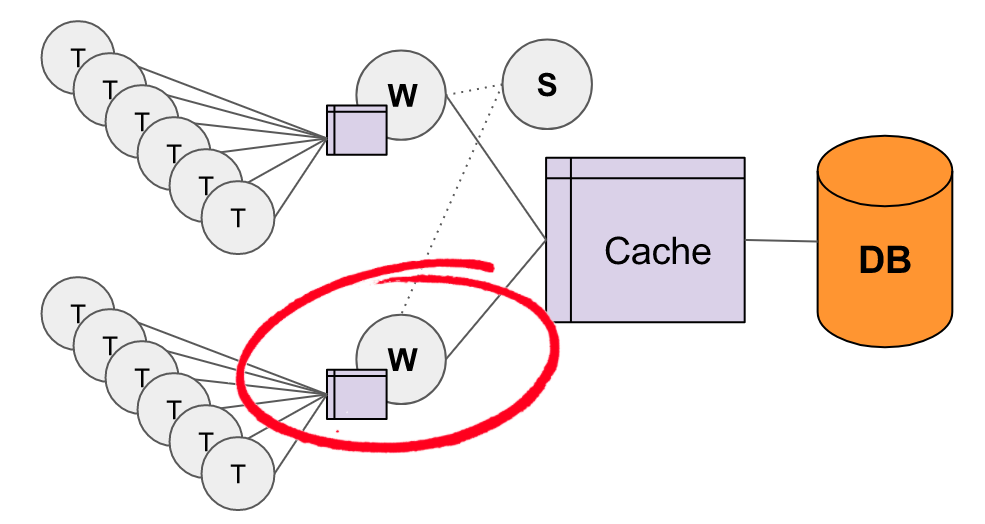
\includegraphics[width=0.5\textwidth]{figures/parsplice.png}\\
\caption{The ParSplice architecture has a storage hierarchy of caches (boxes) and a
dedicated cache process (large box) backed by a persistent database (DB). A splicer
(S) tells workers (W) to generate segments and workers employ tasks (T) for more
parallelization. We focus on the worker's cache (circled), which facilitates
communication and segment exchange between the worker and its tasks.
\label{fig:parsplice}}
\end{figure}

ParSplice~\cite{perez:jctc20150parsplice} is an accelerated molecular dynamics
(MD) simulation package developed at LANL. It is part of the Exascale Computing
Project\footnote{http://www.exascale.org/bdec/} and is important to LANL's
Materials for the Future initiative. 

\subsection{Background}

As shown in Figure~\ref{fig:parsplice}, the phases are:

\begin{enumerate}

  \item a splicer tells workers to generate segments (short MD trajectory) for
  specific states

  \item workers read initial coordinates for their assigned segment from data
  store; the key-value pair is (state ID, coordinate)

  \item upon completion, workers insert final coordinates for each segment into
  data store, and wait for new segment assignment

\end{enumerate}

The computation can be parallelized by adding more workers or by adding tasks
to parallelize individual workers.  The workers are stateless and read initial
coordinates from the data store each time they begin generating segments. Since
worker tasks do not maintain their own history, they can end up reading the
same coordinates repeatedly. To mitigate the consequences of these repeated
reads, ParSplice provisions a hierarchy of caches that sit in front of a single
persistent database.  Values are written to each tier and reads traverse up the
hierarchy until they find the data.  

We use ParSplice to simulate the evolution of metallic nanoparticles that grow
from the vapor phase.  This simulation stresses the storage hierarchy more than
other input decks because it uses a cheap potential, has a small number of
atoms, and operates in a complex energy landscape with many accessible states.
As the run progresses, the energy landscape of the system becomes more complex
and more states are visited.  Two domain factors control the number of entries
in the data store: the growth rate and the temperature. The growth rate
controls how quickly new atoms are added to the nanoparticle: fast growth rates
lead to non-equilibrium conditions, and hence increase the number of states
that can be visited.  However, as the particle grows, the simulation slows down
because the calculations become more expensive, limiting the rate at which new
states are visited.  On the other hand, the temperature controls how easily a
trajectory can jump from state to state; higher temperatures lead to more
frequent transitions but temperatures that are too high result in meaningless
simulations because trajectories have so much energy that they are equally
likely to visit any random state. 

%IT HAS 8K keys!  How did we take these measurements
\subsection{Experimental Setup}

We instrumented ParSplice with performance counters and keyspace counters.  The
performance counters track ParSplice progress while keyspace counters track
which keys are being accessed by the ParSplice ranks. Because the keyspace
counters have high overhead we only turn them on for the keyspace analysis.

All experiments ran on Trinitite, a Cray XC40 with 32 Intel Haswell 2.3GHz
cores per node.  Each node has 128GB of RAM and our goal is to limit the size
of the cache to 3\% of RAM. Note that this is an addition to the 30GB that
ParSplice uses to manage other ranks on the same node.  The scalability
experiment uses 1 splicer, 1 persistent database, 1 cache process, and up to 2
workers. We scale up to 1024 tasks, which spans 32 nodes and disable
hyper-threading because we experience unacceptable variability in performance.
For the rest of the experiments, we use 8 nodes, 1 splicer, 1 persistent
database, 1 cache process, 1 worker, and up to 256 tasks.  The keyspace
analysis that follows is for the cache on the worker node, which is circled in
Figure~\ref{fig:parsplice}.  


\subsection{Results and Observations}
\label{sec:parsplice-keyspace-analysis}

\begin{figure}[t]
  \noindent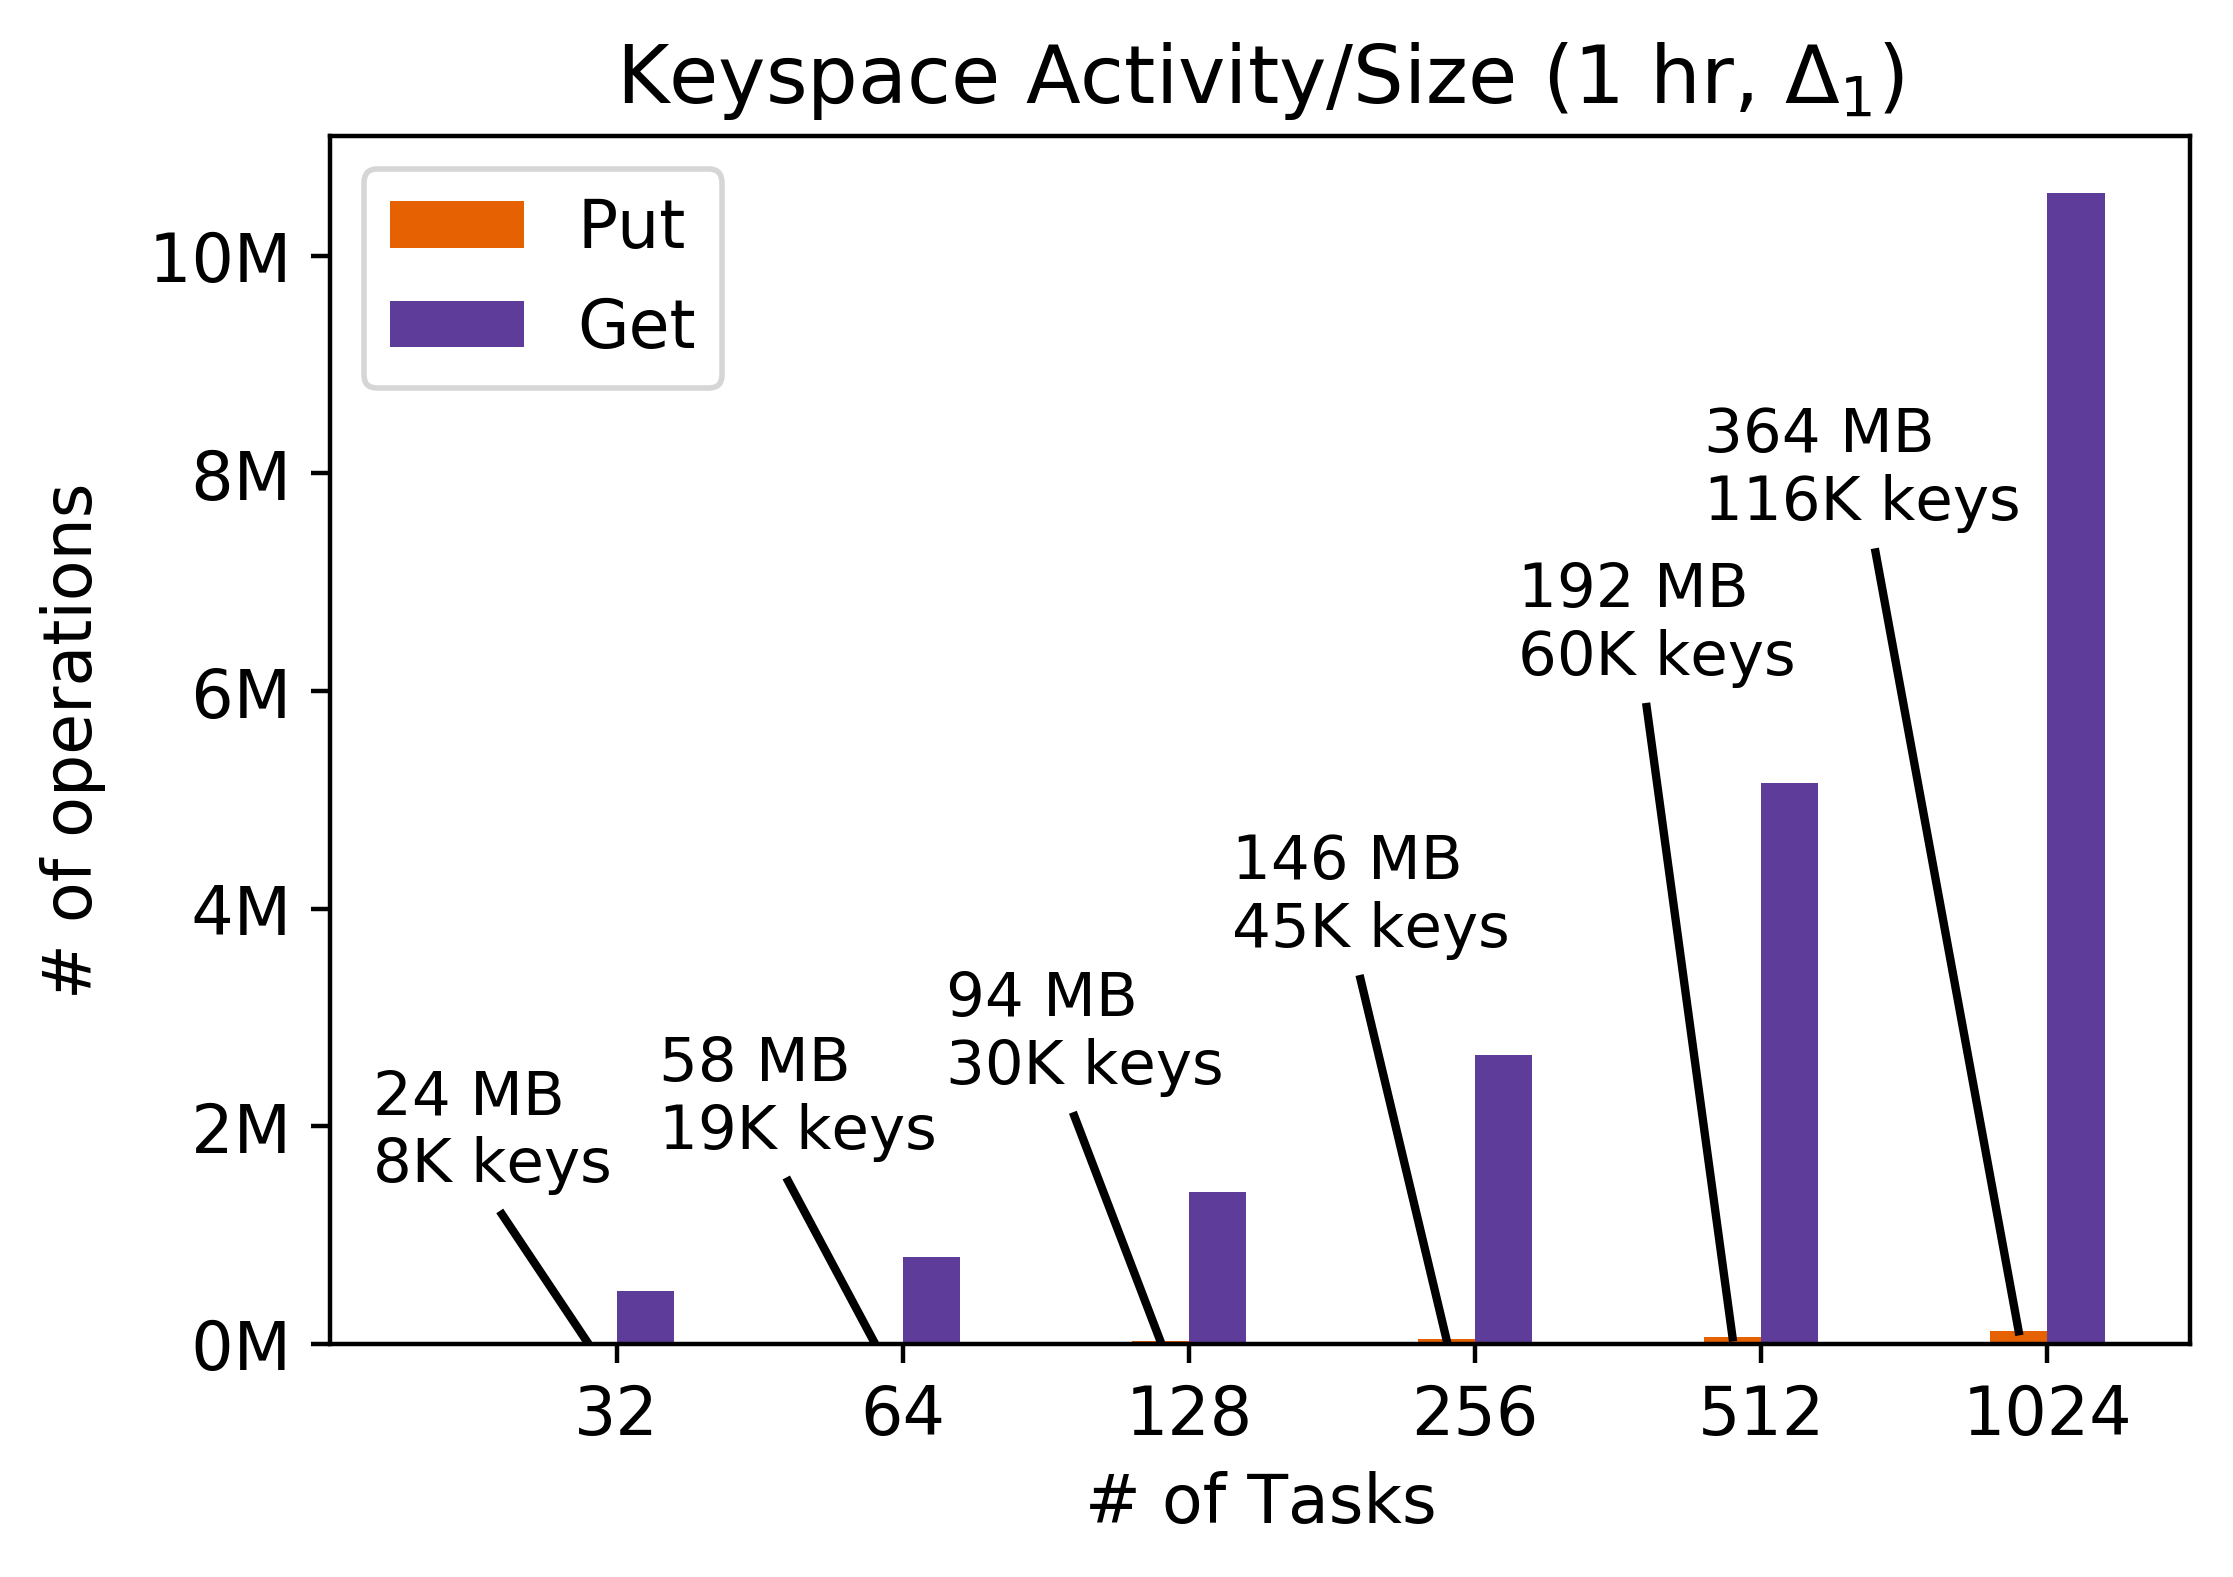
\includegraphics[width=0.5\textwidth]{figures/methodology-keyspace.png}\\
  \caption{The keyspace is small but must satisfy many reads as workers
  calculate segments. Memory usage scales linearly, so it is likely that we will need
  more than one node to manage segment coordinates when we scale the system or jobs up.
  \label{fig:methodology-keyspace}}
\end{figure}

Our analysis shows that ParSplice accesses keys in a structured and predictable
way. The following 4 observations shape the policies we design later in the
paper.

\subsubsection{\underline{Scalability}} Figure~\ref{fig:methodology-keyspace} shows the
keyspace size (text annotations) and request load (bars) after a one hour run
with a different number of tasks (\(x\) axis). While the keyspace size and
capacity is modest the memory usage scales linearly with the number
of tasks, which is a problem if we want to scale to Trinitite's 3000 cores.
Furthermore, the size of the keyspace also increases linearly with the length
of the run.  Extrapolating these results puts an 8 hour run across all 100
Trinitite nodes at 8GB for one cache.  This memory utilization easily eclipses
the 3\% memory usage per node threshold we set earlier, even without factoring
in the usage from other workers.

\subsubsection{\underline{An active but small keyspace}}

The bars in Figure~\ref{fig:methodology-keyspace} show \(50-100\times\) as many
reads (\texttt{get()}) as writes (\texttt{put()}).  Tasks read the same key for
extended periods because the trajectory gets stuck in so-called superbasins
composed of tightly connected sets of states.  Writes only occur for the final
state of segments generated by tasks; their magnitude is smaller than reads
because the caches ignore redundant write requests. 

\begin{figure}[t]
  \noindent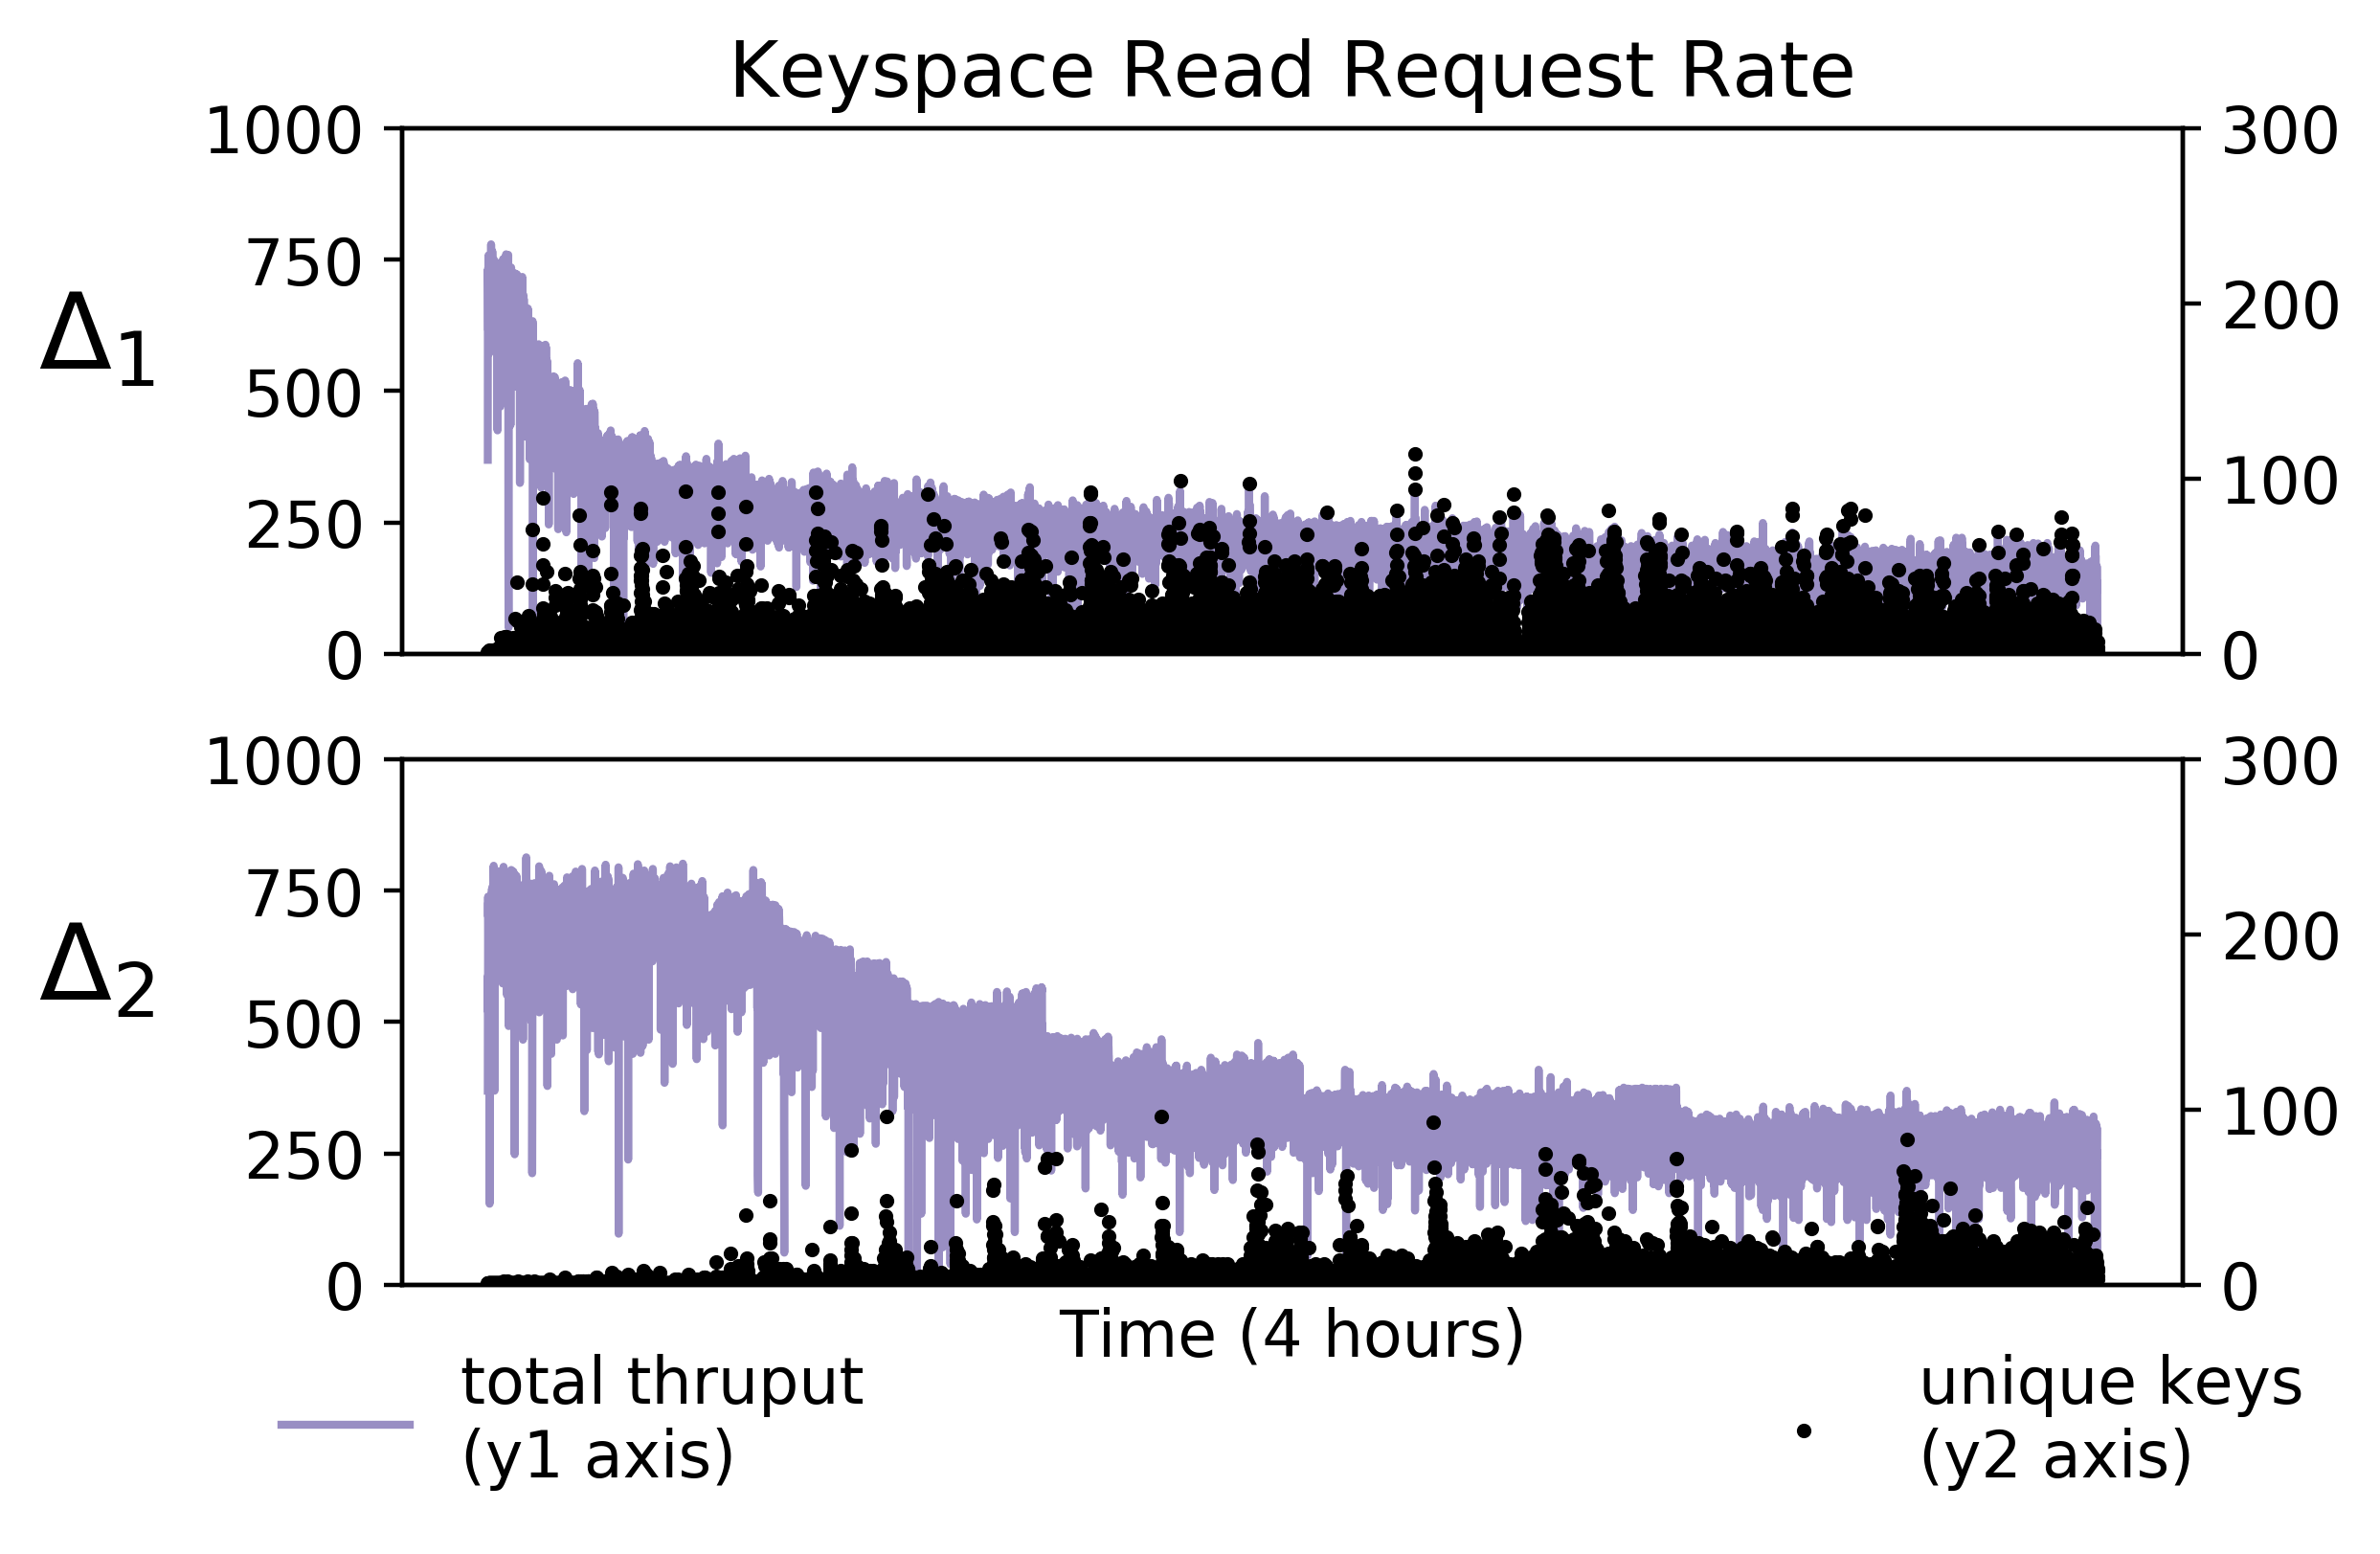
\includegraphics[width=0.5\textwidth]{figures/motivation-regimes.png}\\
  \caption{Key activity for ParSplice starts with many reads to a small set of
keys and progresses to less reads to a larger set of keys.  The line shows the
rate that EOM minima values are retrieved from the key-value store (\(y1\)
axis) and the points along the bottom show the number of unique keys accessed in a 1
second sliding window (\(y2\) axis). Despite having different growth rates
(\(\Delta\)), the structure and behavior of the key activities are similar.
\label{fig:motivation-regimes}}
\end{figure}

\subsubsection{\underline{Initial conditions influence key activity}}
Figure~\ref{fig:motivation-regimes} shows how ParSplice tasks read key-value
pairs from the worker's cache for two different initial conditions of
\(\Delta\), which is the rate that new atoms enter the simulation.  The line is
the read request rate (\(y1\) axis) and the dots along the bottom are the
number of unique keys accessed (\(y2\) axis).  The access patterns for
different growth rates have temporal locality, as the reads per second for
\(\Delta_2\) look like the reads per second for \(\Delta_1\) stretched out
along the time axis.  The \(\Delta_1\) growth rate adds atoms every 100K
microseconds while the \(\Delta_2\) growth rate adds atoms every 1 million
microseconds. So \(\Delta_2\) has a smaller growth rate resulting in hotter
keys and a smaller keyspace.  Values smaller than \(\Delta_2\)'s growth rate or
a temperature of 400 degrees result in very little database activity because
state transitions take too long. Similarly, values larger than \(\Delta_1\)'s
growth rate or a temperature of 4000 degrees result in an equally meaningless
simulation as transitions are unrealistic.  

This figure demonstrates that small changes to \(\Delta\) can have a strong
effect on the timing and frequency with which new EOM minima are discovered and
referenced.  Trends also exist for temperature and number of workers but are
omitted here for space.  This finding suggests that we need a flexible policy
language and engine to explore these trade-offs.  

\begin{figure}[t]
  \noindent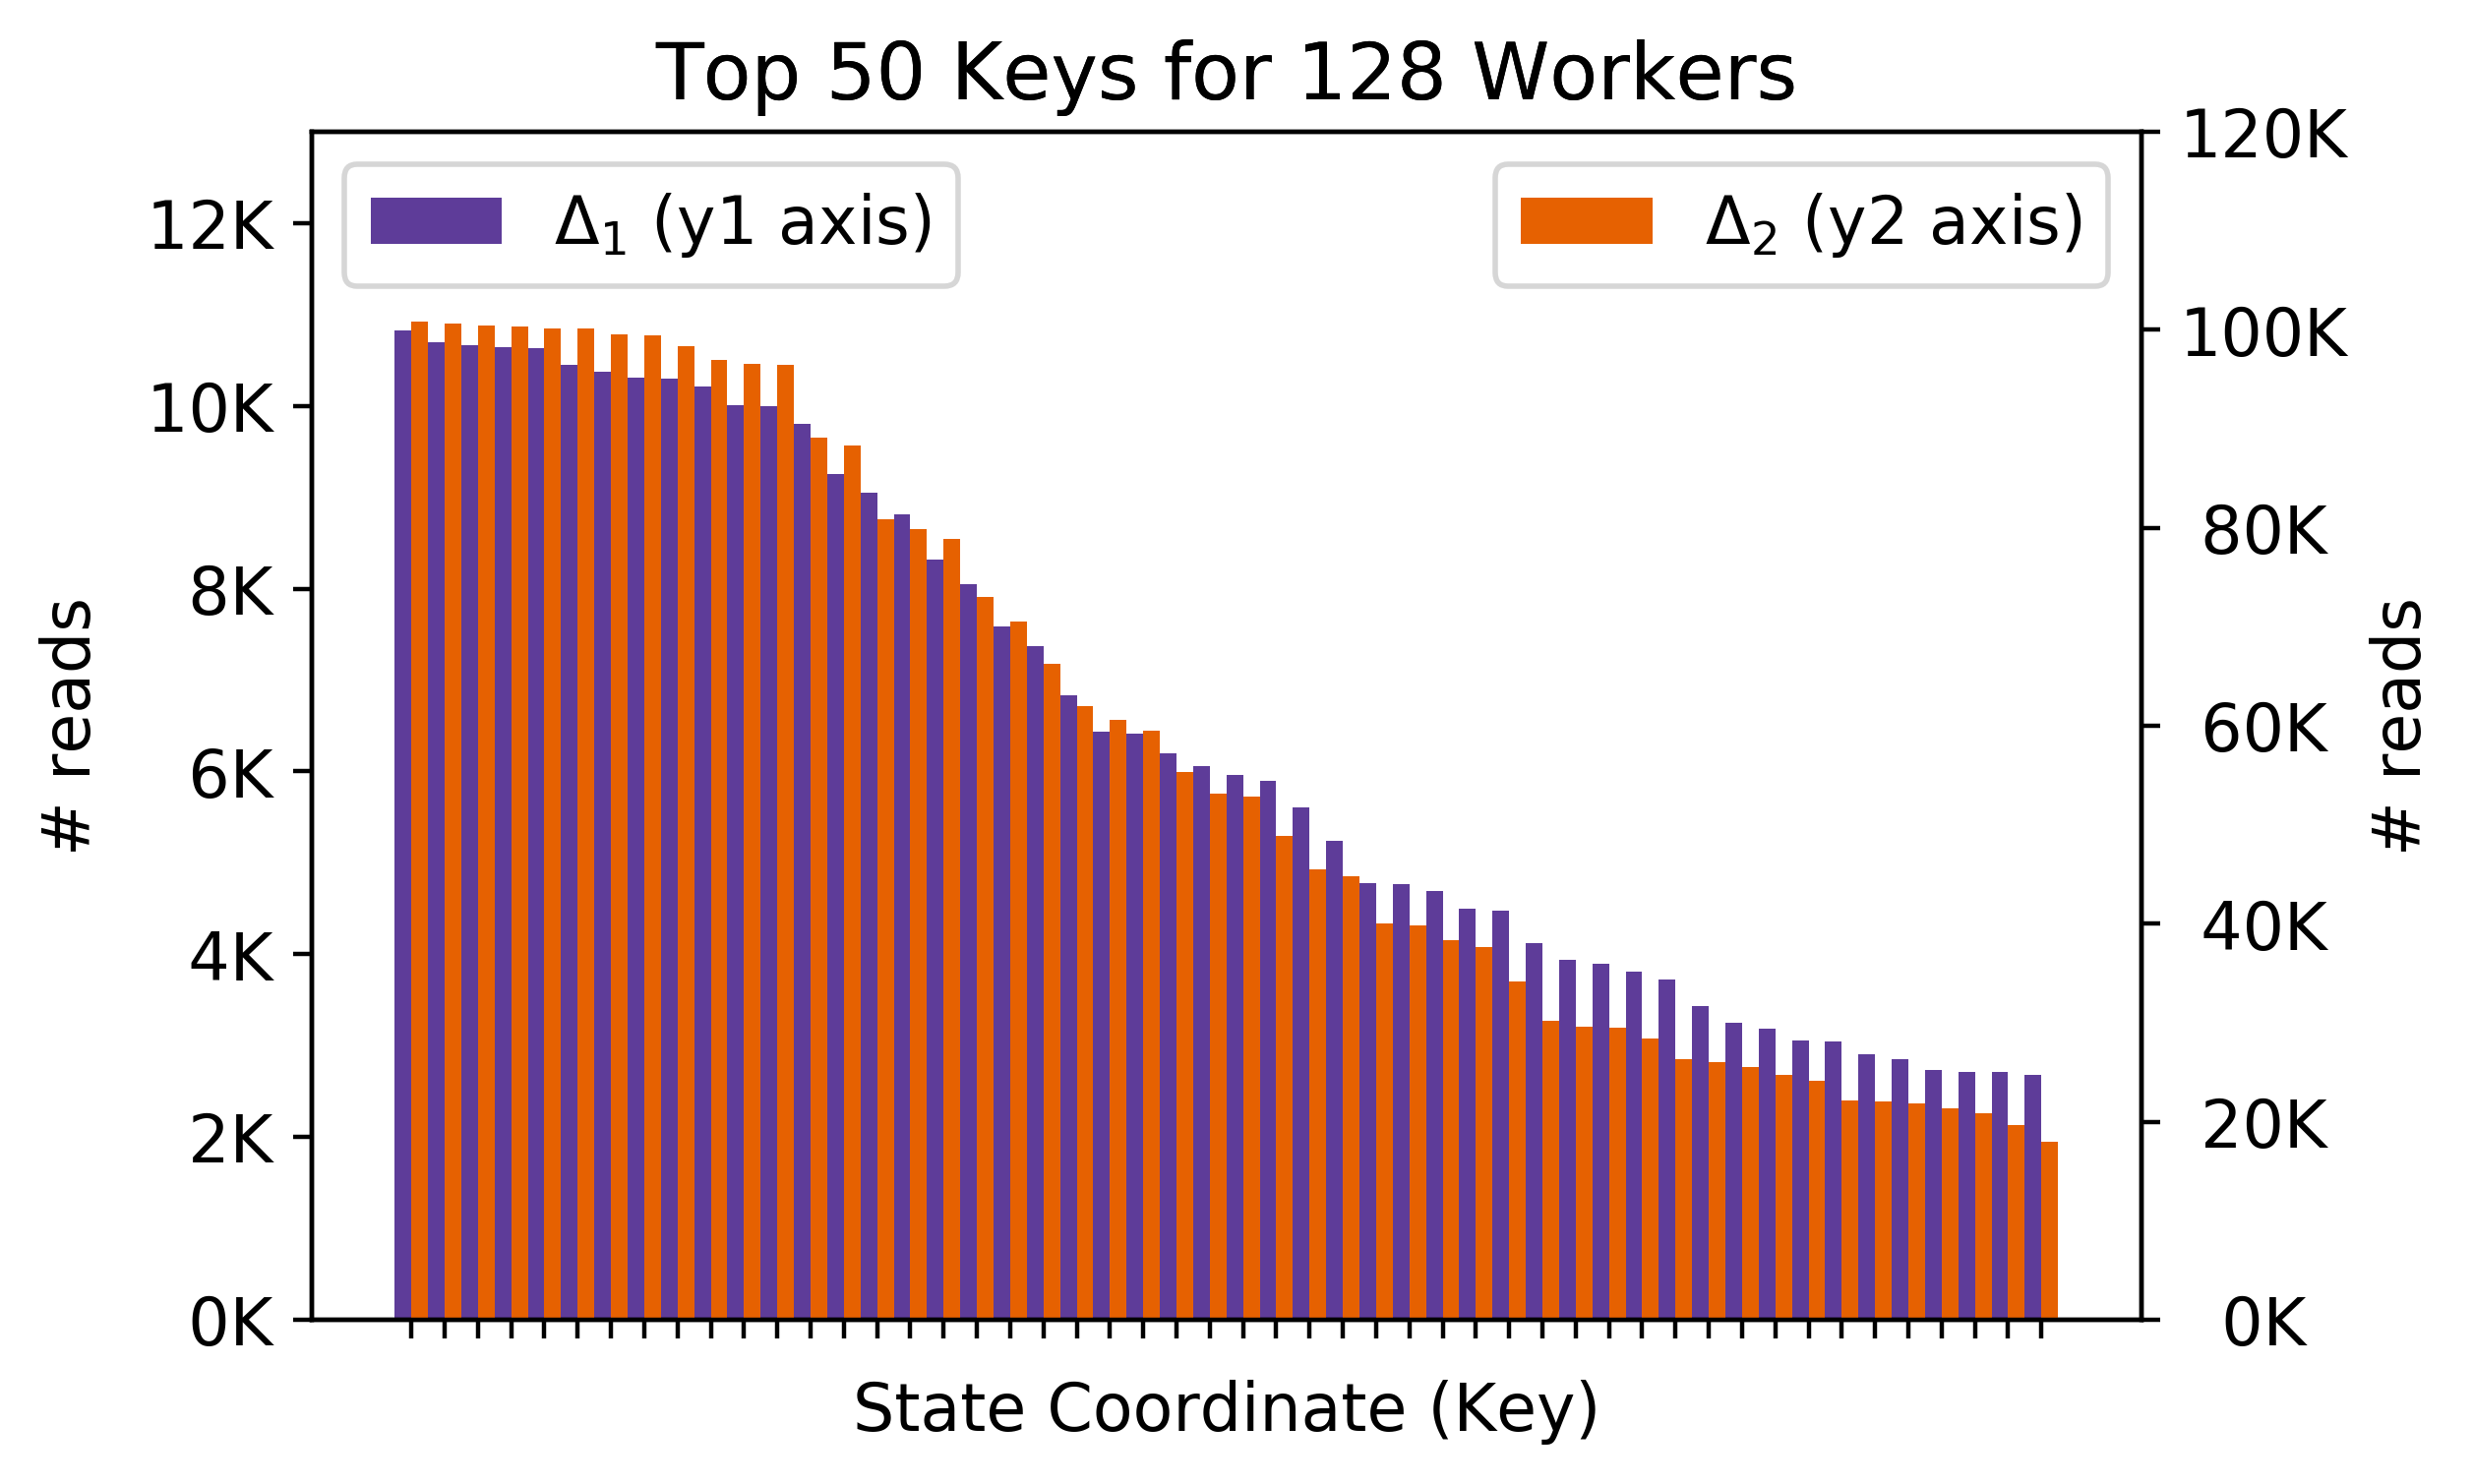
\includegraphics[width=0.5\textwidth]{figures/methodology-keys.png}\\
  \caption{Over time, tasks start to access a larger set of keys resulting in
some keys being more popular than others.  Despite different growth rates
(\(\Delta\)), the spatial locality of key accesses is similar between the two
runs.  ({\it e.g.}, some keys are still read 5 times as many times others).
\label{fig:methodology-keys}}
\end{figure}

\subsubsection{\underline{Entropy increases over time}} The reads per second in
Figure~\ref{fig:motivation-regimes} show that the number of requests decreases
and the number of active keys increases over time.  The number of read and
write requests are highest at the beginning of the run when tasks generate
segments for the same state, which is computationally cheap (this motivates
Section~\S\ref{sec:arch-specific}).  The resulting key access imbalance for the
two growth rates in Figure~\ref{fig:motivation-regimes} are shown in
Figure~\ref{fig:methodology-keys}, where reads are plotted for each unique
state, or key, along the \(x\) axis. Keys are more popular than others (up to
\(5\times\)) because worker tasks start generating states with different
coordinates later in the run.  Figure~\ref{fig:methodology-keys} also shows that the
number of reads changes with different initial conditions (\(\Delta\)), but
that the spatial locality of key accesses is similar ({\it e.g.}, some keys are
still \(5\times\) more popular than others).

\section{Mantle Engine: Methodology}

\subsection{Experimental Setup}

\subsection{Mantle: Dynamic Load Balancing Policies}

%  \item motivation: Mochi load balancer microservice

%  \item background: CephFS implementation

%  \item library architecture, callbacks, environment
We extract Mantle as a library that is linked into a service ({\it e.g.}, file
system, key-value store, application), where administrators program policies
that are embedded into the runtime.  The service needs to be modified to (1)
provide environment of metrics (2) identify where policies are set. At runtime,
Mantle executes the admin's policies for when/where/how much and returns a
decision.

\begin{figure}[t]
  \noindent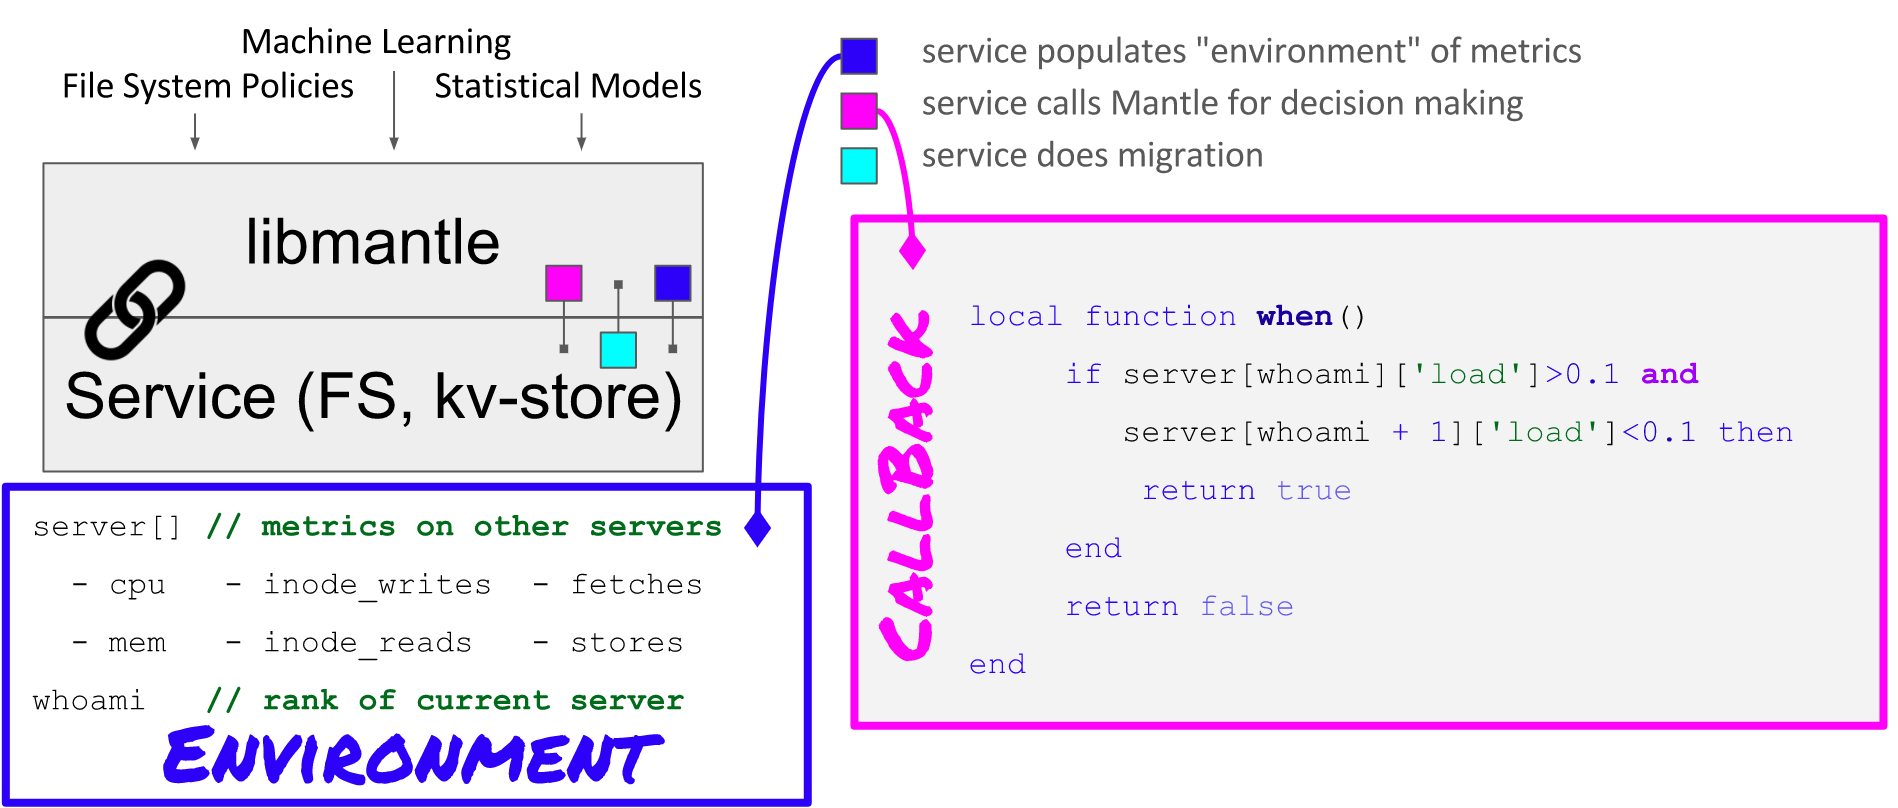
\includegraphics[width=0.5\textwidth]{figures/mantle.png}\\

  \caption{Extracting Mantle as library.\label{fig:mantle}}

\end{figure}

\begin{table}
  \centering
  \begin{tabular}{ r | l | l }
  Metrics     & Data Structure & Description \\\hline
  Cluster     & \{server \(\rightarrow\) \{metric \(\rightarrow\) val\}\}
              & resource util. for servers \\
  Time Series & [(ts, val), ..., (ts, val)]
              & accesses by timestamp (ts) \\
  && \\
              & Service      & Example \\\hline
  Cluster     & File Systems & CPU util., Inode RDs \\
              & ParSplice    & CPU util., Cache Size \\
  Time Series & File Systems & Accesses to directory \\
              & ParSplice    & Accesses to key in DB\\
  \end{tabular}
  \caption{Types of metrics exposed by the service to the policy engine using Mantle.\label{table:metrics}}
\end{table}

%of timestamp (ts), value pairs representing accesses over time types of
%metrics: key value pairs
Services expose two types of metrics with Mantle: cluster metrics for
describing resource utilization and time series metrics for describing accesses
over time. Table~\ref{table:metrics} shows how these metrics are accessed from
the policies written by administrators. Cluster metrics are read from a
dictionary indexed by server and metric name, where server is a node identifier
({e.g.}, MPI Rank, metadata server name), metric is a resource name and val is
the current reading for that metric.  Examples of \texttt{(metric, value)}
pairs are CPU or memory pressure, as shown in Figure~\ref{fig:mantle}.  For
time series metrics, the service passes a pointer to an array of
\texttt{(timestamp, value)} pairs. We use a pointer so we can pass a large
number of values, like accesses over time to a database or directory in the
file system namespace, but this limits the time series metrics to only include
values from the {\it current } node.

% policies themselves
Administrators write policies as callbacks that use the metrics from above.
Figure~\ref{fig:mantle} shows an example policy for the ``when()" callback, where the
current server (\texttt{whoami}) migrates load if it is has load
(\texttt{>0.1}) and if its neighbor server (\texttt{whoami + 1}) does not have
load (\texttt{<0.1}). 

\subsection{Integrating Mantle into ParSplice}

\begin{itemize}
  \item providing environment of metrics
  \item identifying where policies are made
\end{itemize}

%\subsection{Trajectory Length}
%
%\subsection{Cloud Techniques: Elastic Search}
%
%What if we re-provision resources in response to events outside the
%application's control, such as a slow Lustre.
%
%\subsection{Future work}
%
%How Much: cache policy from past, regime detection, Belady's Min

\section{Cache Management Using Storage System Architecture Knowledge}
\label{sec:arch-specific}

Using the Mantle policy engine, we test a variety of cache management 
algorithms on the worker using the keyspace analysis in
Section~\S\ref{sec:parsplice-keyspace-analysis}.  Our evaluation uses the total
``trajectory length" as the goodness metric. This value is the duration of the
overall trajectory produced by ParSplice. At ideal efficiency, the trajectory
length should increase with the square root of the wall-clock time, since the
wall-clock cost of time-stepping the system by one simulation time unit
increases in proportion of the total number of atoms.  The policy should avoid
reducing the trajectory length and be fast enough to run as often as we want to
detect key access patterns.  First we size the cache according to our system
specific knowledge, {\it i.e.} the hardware and software of the storage
hierarchy.

% technical details
We implement a basic LRU cache using a ``when" policy of:
\texttt{server[whoami]['cachesize']>n} and a ``how much" policy of
\texttt{servers[whoami]['cachesize']-n}.  The results for different cache sizes
for a growth rate of \(\Delta_1\) over a 2.5 hour run across 256 workers is
shown in Figure~\ref{fig:methodology-tradeoff}.  ``Baseline" is the performance
of unmodified ParSplice  measured in trajectory duration (\(y1\) axis) and
utilization is measured with memory footprint of just the cache (\(y2\) axis).
The middle graph labeled ``Fixed Cache Size" shares the \(y\) axes and shows
the trade-off of using a basic LRU-style cache of different sizes, where the
penalty for a cache miss is retrieving the data from the persistent database.
The error bars are the standard deviation of 3 runs.  Although the keyspace
grows to 150K, a 100K key cache achieves 99\% of the performance. Decreasing
the cache degrades performance and predictability.

%\begin{figure}[h] \footnotesize \begin{minted}{lua}
%server[whoami]['cachesize'] > n \end{minted} \end{figure}

%and ``how much":
%\begin{figure}[h]
%\footnotesize
%\begin{minted}{lua}
%servers[whoami]['cachesize'] - n
%\end{minted}
%\end{figure}


\begin{figure}[t]
\noindent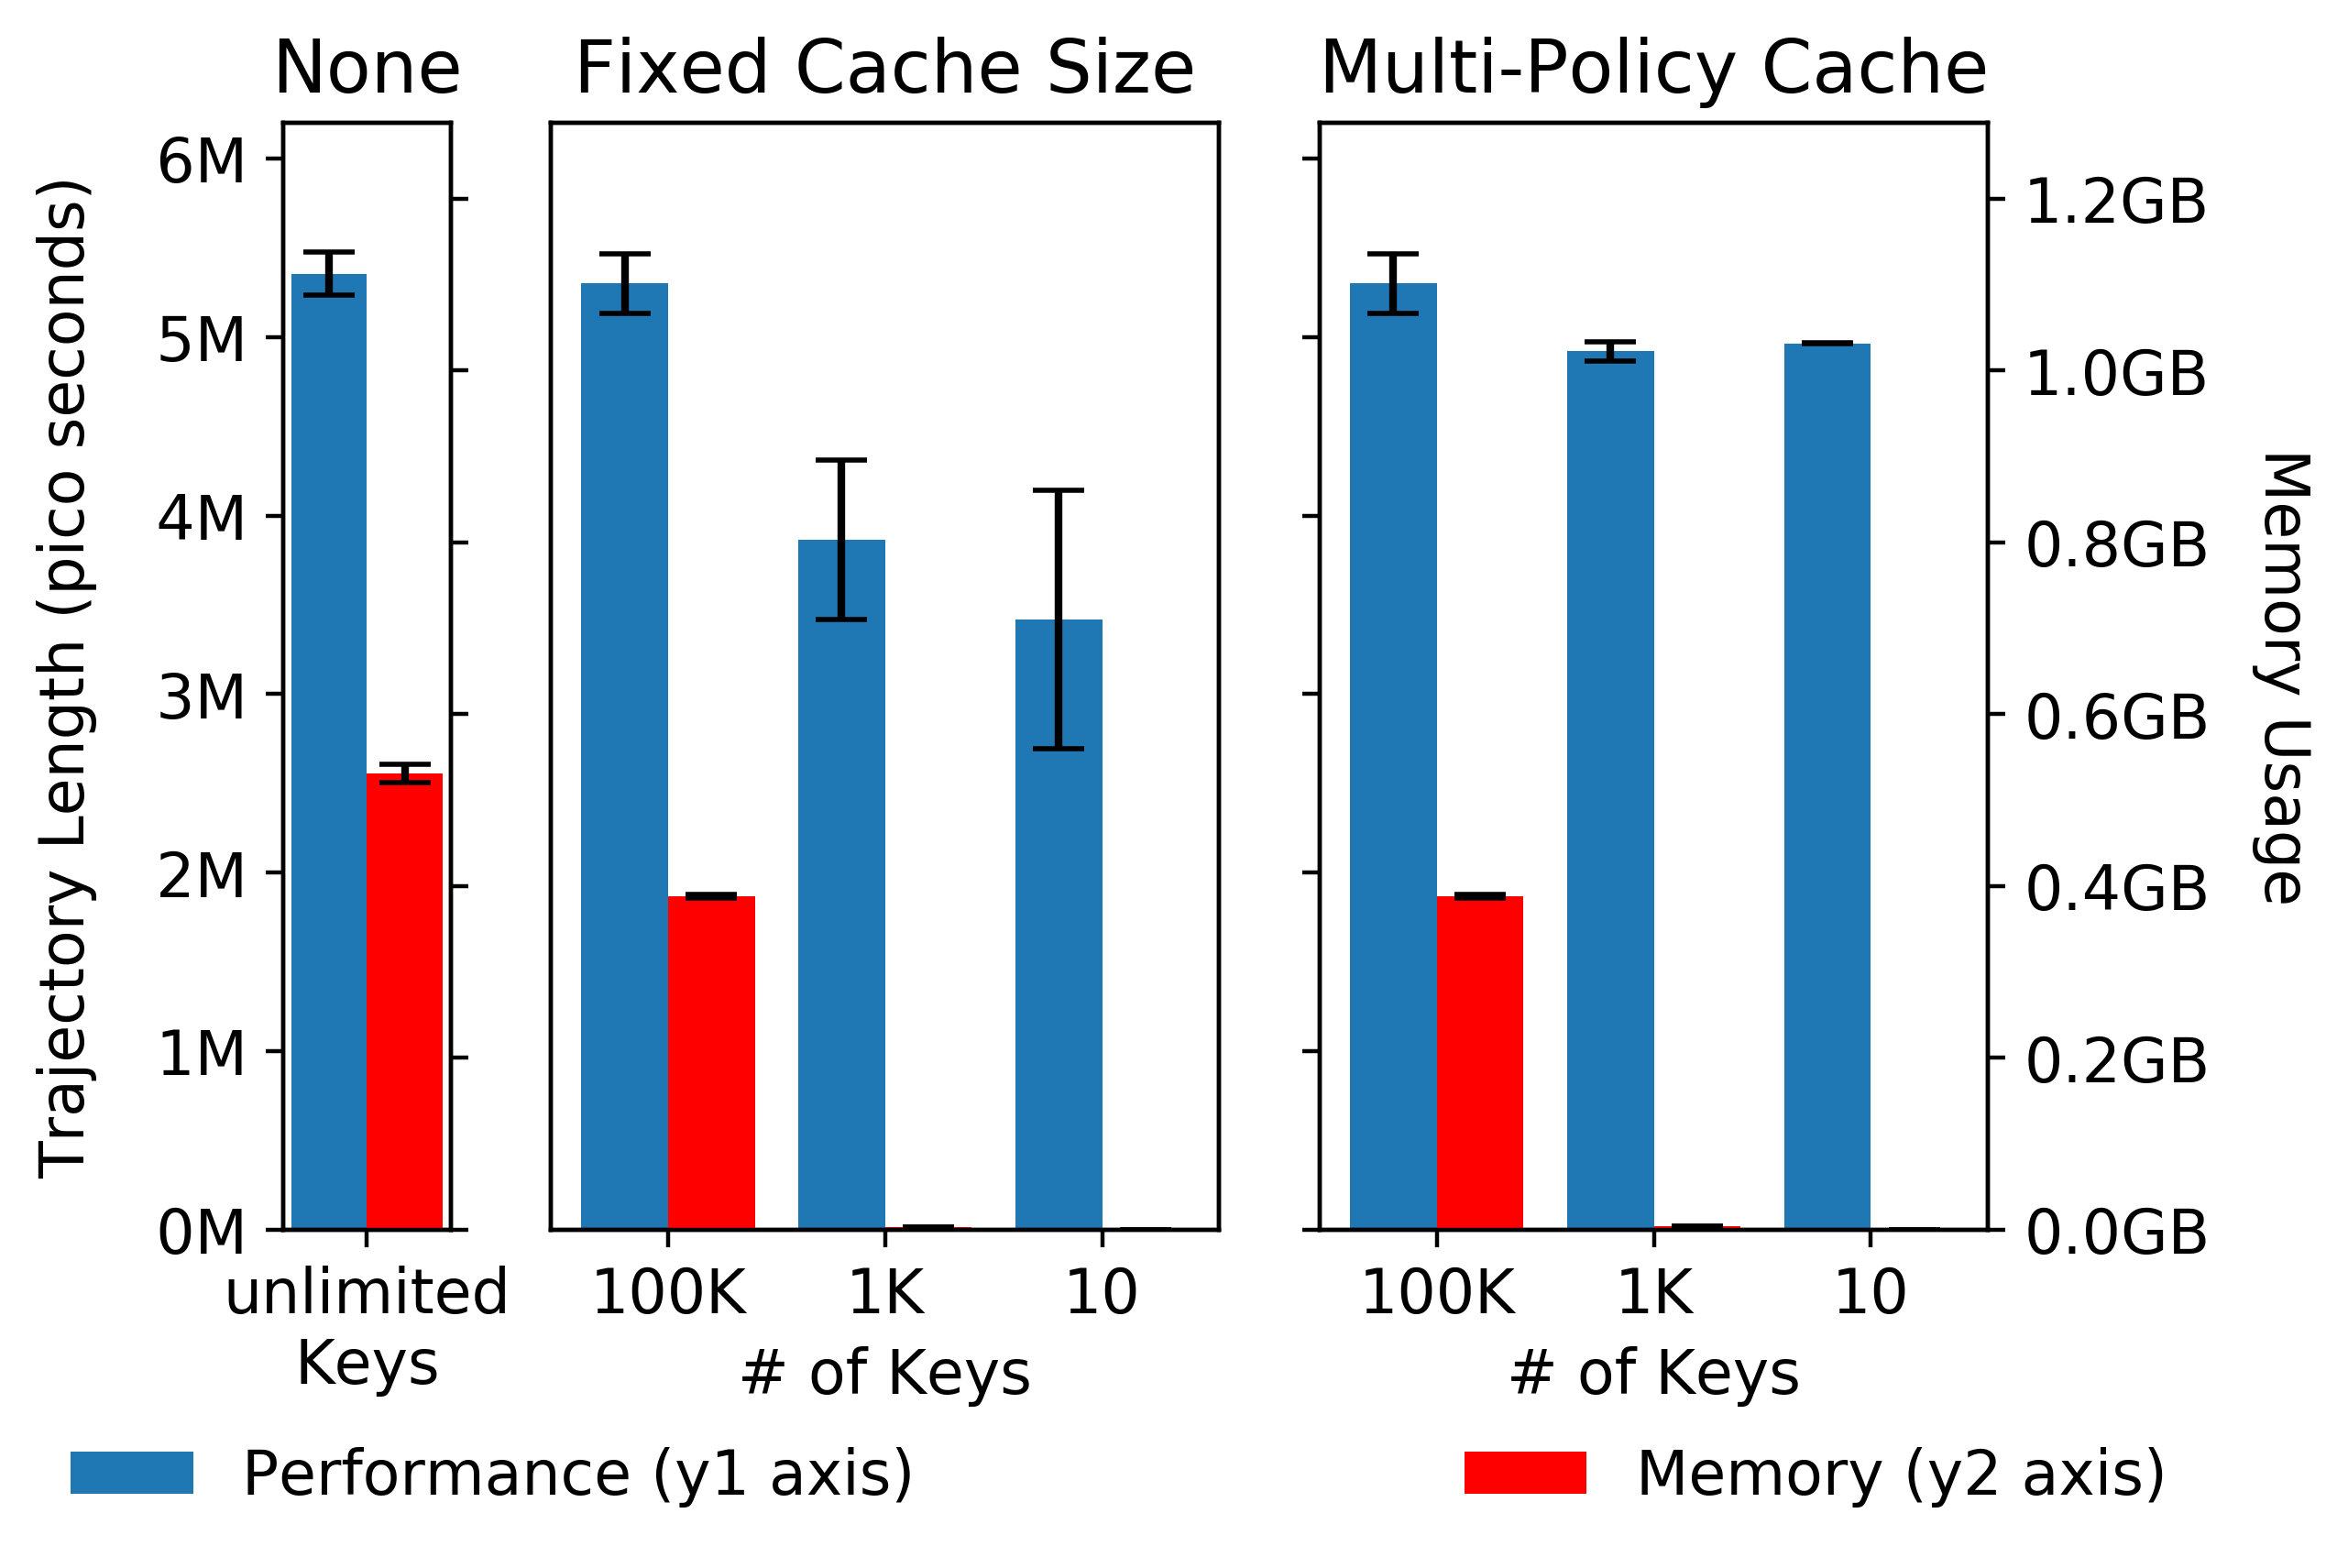
\includegraphics[width=0.5\textwidth]{figures/methodology-tradeoff.png}\\
\caption{Policy performance/utilization shows the trade-offs of different sized
caches (\(x\) axis).  ``None" is ParSplice unmodified, ``Fixed Sized Cache"
evicts keys using LRU, and ``Multi-Policy Cache" switches to fixed sized cache
after absorbing the workload's initial burstiness. This parameter sweep
identifies the ``Multi-Policy Cache" of 1K keys as the best solution but this
only works for this system setup and initial configurations.
 \label{fig:methodology-tradeoff}}
\end{figure}

\begin{figure}[t]
        \centering
        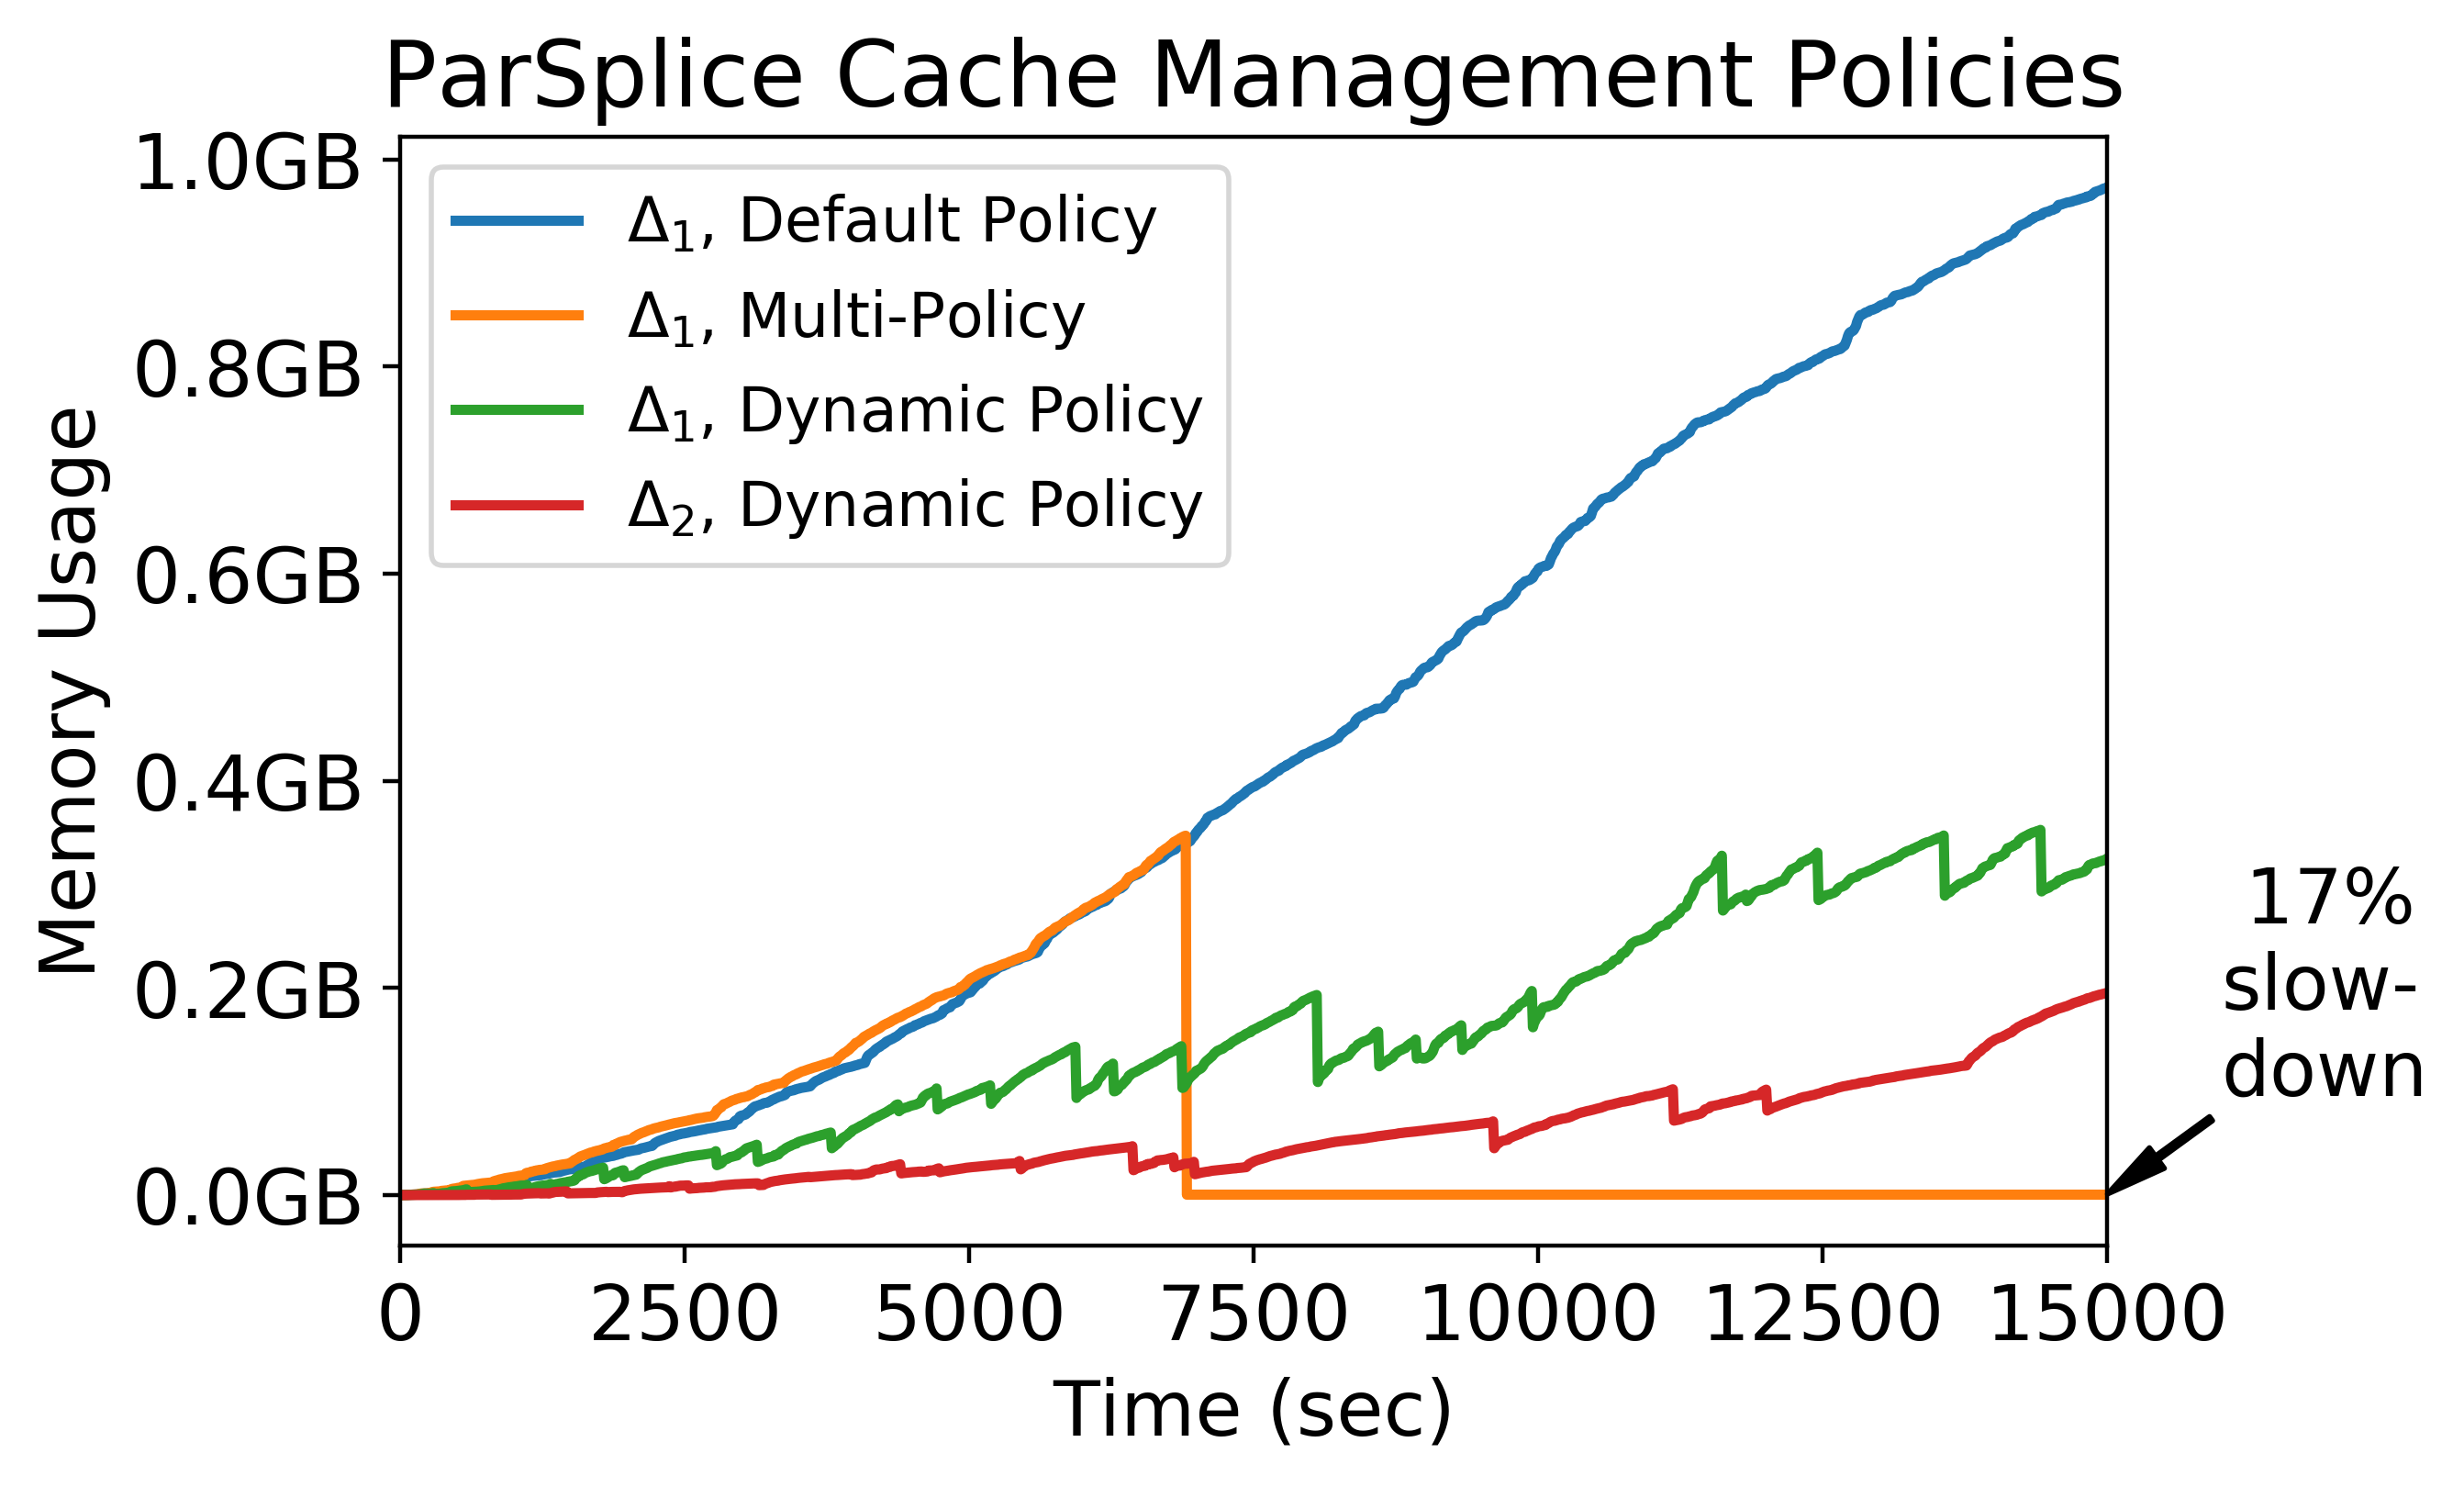
\includegraphics[width=0.5\textwidth]{figures/memory-vs-time.png}\\
	\caption{Memory utilization for ``No Cache Management" (unlimited cache
growth), ``Multi-Policy" (absorbs initial burstiness of workload), and
``Dynamic Policy" (sizes cache according to key access patterns). The dynamic
policies saves the most memory without sacrificing performance.
\label{fig:memory-vs-time}}
\end{figure}%
 


%
%\footnotesize \centering \begin{minted}[xleftmargin=3em,linenos]{lua} function
%when() if server[whoami]['cachesize'] > n then return true end return false
%end
%
%function howmuch() if servers[whoami]['cachesize'] > n return
%servers[whoami]['cachesize'] - n end return 0 end \end{minted} \caption{Policy
%that implements a basic LRU cache. The performance and memory utilization for
%different values of \(n\) are graphed in
%Figure~\ref{fig:methodology-tradeoff}.  \label{src:lru}} \end{figure}

% why is the performance lower for smaller caches?
But the top graph in Figure~\ref{fig:motivation-regimes} suggests that a
smaller cache size should suffice, as only 100 keys seem to be active at any
one time.  It turns out that the unique keys plotted in
Figure~\ref{fig:motivation-regimes} are per second and are not representative
of the actual active keyspace; the number of active keys is larger than 100, as
some keys may be accessed at time \(t_0\), not in \(t_1\), and then again in
\(t_2\). Because the cache is too small, reads and writes fall through to the
rest of the storage hierarchy and the excessive traffic triggers a LevelDB
compaction on the persistent database.  To avoid these compactions, which
temporarily block operations, we design a multi-policy cache that switches
between:

\begin{itemize}
  \item unlimited growth policy: cache increases on every write
  \item \(n\) key limit policy: cache constrained to \(n\) keys
\end{itemize}

% results: same level of performance can be achieved 
The key observation is that small caches incur too much load on the persistent
database at the beginning of the run but should suffice after the initial read
flash crowd passes because the keyspace is far less active.  We program Mantle
to trigger the policy switch at 100K keys to absorb the flash crowd at the
beginning of the run. Once triggered, keys are evicted to bring the size of the
cache down to the threshold.  The actual policy is shown and described in more
detail in Section~\S\ref{sec:scope} in Figure~\ref{src:lru-dyn}.  The plot on
the right side of Figure~\ref{fig:methodology-tradeoff} shows the
performance/utilization trade-off of the multi-policy cache, where the cache
sizes for the \(n\) key limit policy are along the \(x\) axis.  The performance
and memory utilization for a 100K key cache size is the same as the 100K bar in
the ``Fixed Cache Size" graph in Figure~\ref{fig:methodology-tradeoff} but the
rest reduce the size of the keyspace after the read flash crowd.  We see the
worst performance when the policy switches to the 10 key limit policy, which
achieves 94\% of the performance while only using 40KB of memory. 

% caveats: it is calculating 90% of the trajectory, memory value reported is final
\subsubsection*{Caveats}

The results in Figure~\ref{fig:methodology-tradeoff} are slightly deceiving for
two reasons: (1) segments take longer to generate later in the run and (2) the
memory footprint is the value at the end of 2.5 hours.  For (1), the trajectory
length vs.  wall-clock time curves down over time; as the nanoparticle grows it
takes longer to generate segments so by the time we reach 2 hours, over 90\% of
the trajectory is already generated.  For (2), the memory footprint rises until
it reaches the 100K key switch threshold at 0.4GB and then reduces to the final
value after switching policies. The memory usage over time for this policy is
shown by the ``\(\Delta_1\), Multi-Policy" curve in
Figure~\ref{fig:memory-vs-time} but in Figure~\ref{fig:methodology-tradeoff} we
plot the final value.  Despite these caveats, the result is still valid: we
found a multi-policy cache management strategy that absorbs the cost of a high
read throughput on a small keyspace and reduces the memory pressure for a 2.5
hour run.  To improve the policy even more, we need a way to identify what
thresholds to use for different system setups ({\it e.g.}, different ParSplice
parameters, number of worker tasks, and job lengths).  

\section{Cache Management Using Application-Specific Knowledge}
\label{sec:dom-specific}

\begin{figure*}[t!]
    \begin{subfigure}[t]{0.48\textwidth}
        \centering
	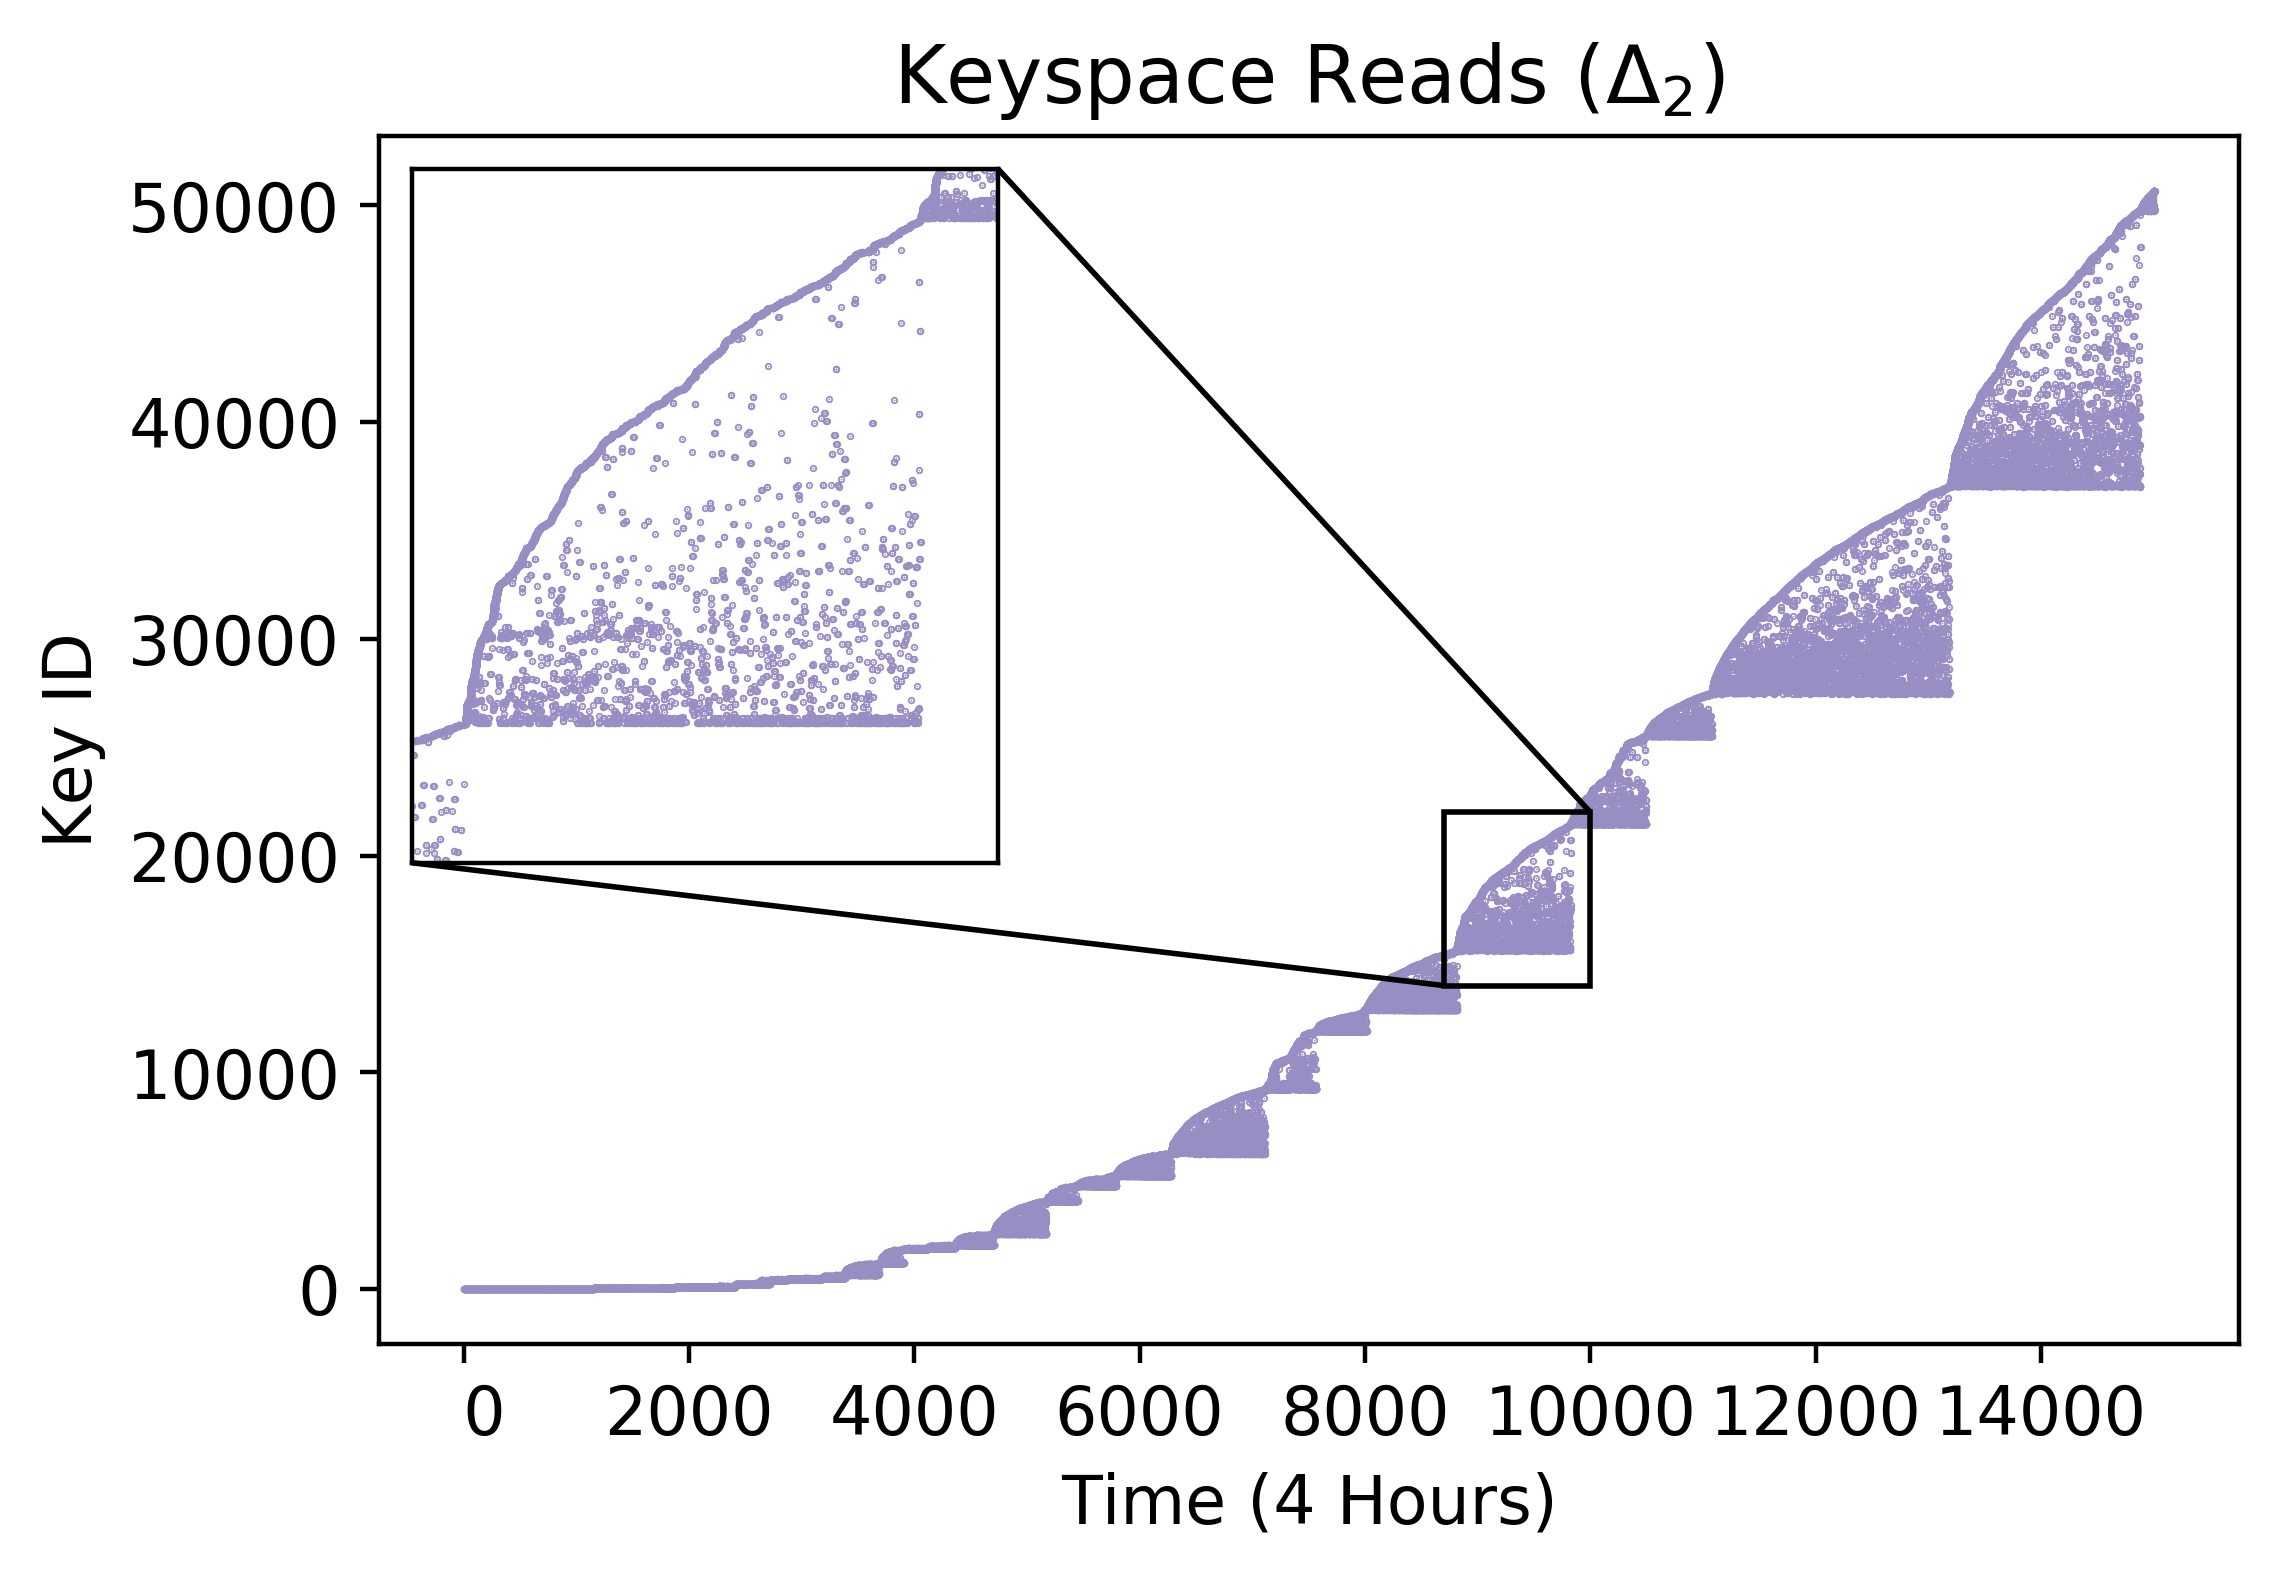
\includegraphics[width=1\textwidth]{figures/keyspace-zoomed.png}\\

\caption{Key activity for a 4 hour run shows groups of accesses to the same
subset of keys. Detecting these access patterns leads to a more accurate cache
management strategy, which is discussed in Section~\S\ref{sec:regime-detection}
and the results are in Figure~\ref{fig:dscache-vs-none}.
\label{fig:keyspace-zoomed}}
    \end{subfigure}%
    ~ 
    \begin{subfigure}[t]{0.48\textwidth}
        \centering
        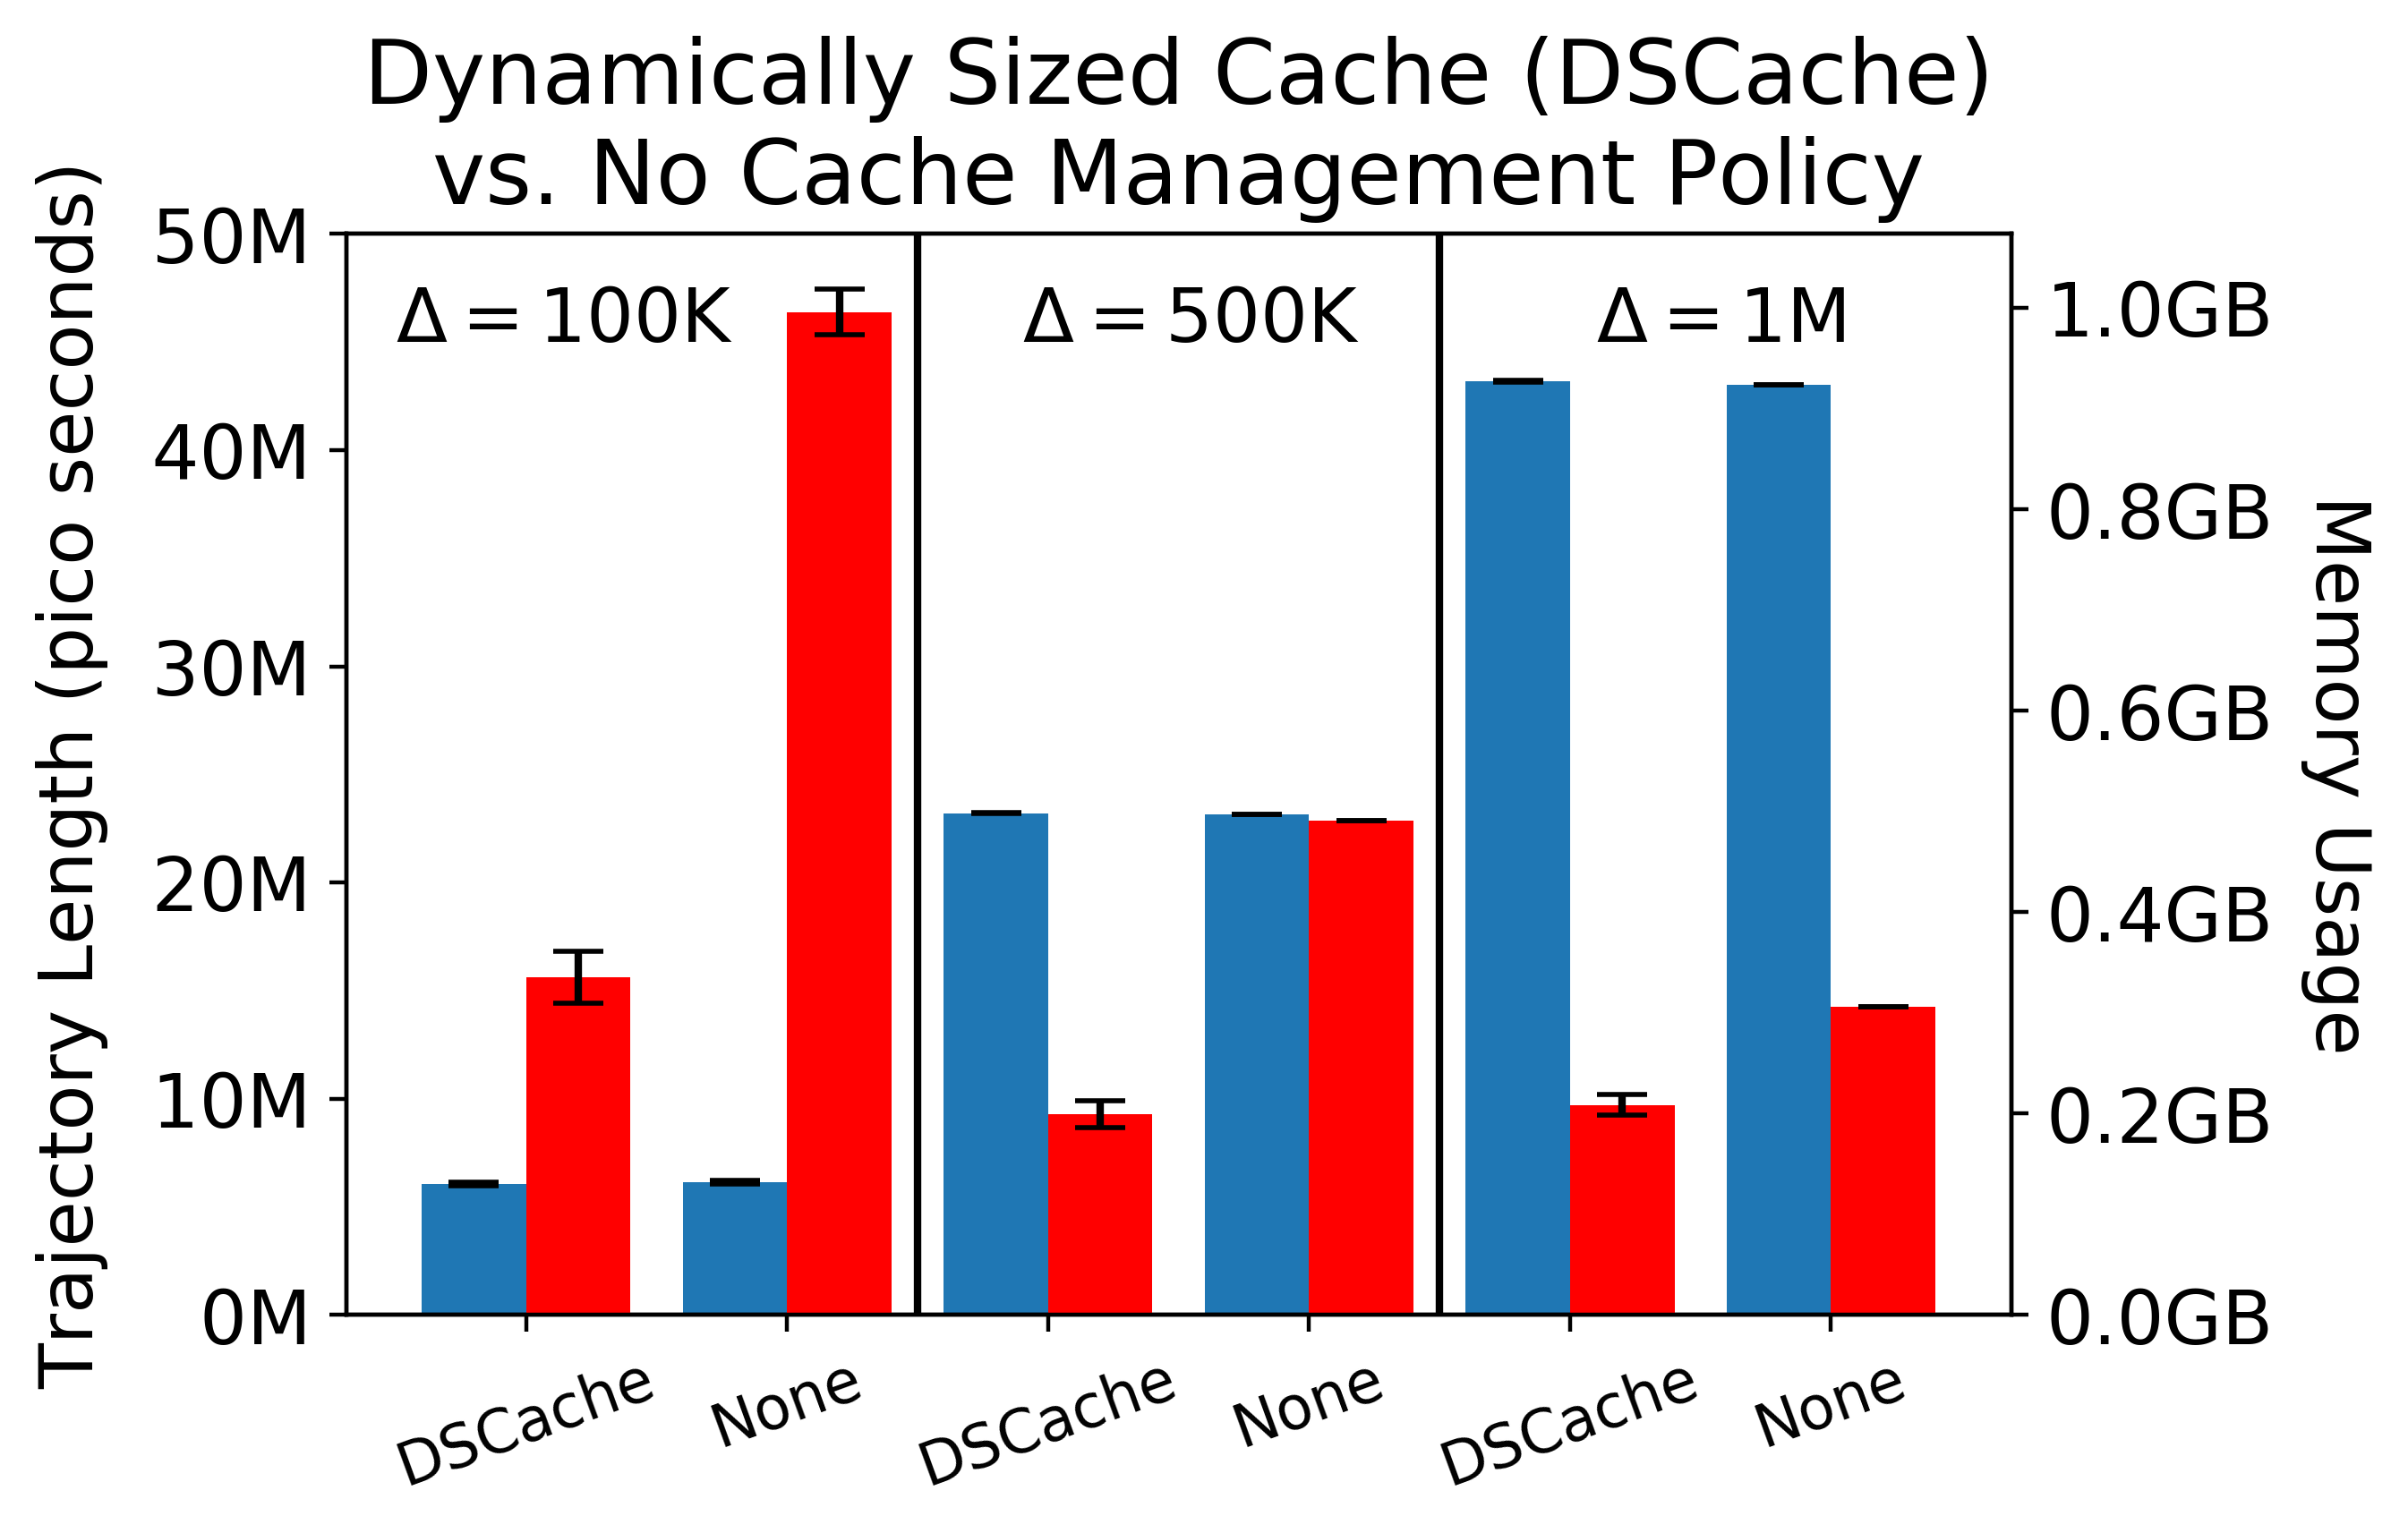
\includegraphics[width=1\textwidth]{figures/dscache-vs-none.png}\\
	\caption{The performance/utilization for the dynamically sized cache (DSCache)
policy. With negligible performance degradation, DSCache adjusts to different initial configurations
(\(\Delta\)s) and saves 3\(\times\) as much memory in the best case.
\label{fig:dscache-vs-none}}
    \end{subfigure}%
    \caption{Different cache management policies tested over the Mantle policy engine.}
\end{figure*}

\begin{figure}[tb]
\footnotesize
\begin{minted}[xleftmargin=3em,linenos]{lua}
d = timeseries()
ts, id = d:get(d:size())
fan  = {start=nil, finish=ts, top=0, bot=id}
fans = {}
for i=d:size(),1,-1 do     -- iterate backwards
  ts, id = d:get(i)
  if id < fan['bot'] then  -- found a new fan!
    fan['start']  = ts
    fans[#fans+1] = fan 
    fan = {start=nil, finish=ts, top=0, bot=id}
  end 

  if id > fan['top'] then  -- track top of fan
    fan['top'] = id 
  end 
end
fan['start'] = 0 
fans[#fans+1] = fan 

if #fans < 2 then -- do not evict current fan
  return false
else
  WRstate(fans[#fans-1]['top']-fans[1]['bot']) 
  return true
end
\end{minted}
\caption{The dynamically sized cache policy iterates backwards over
timestamp-key pairs and detects when accesses move on to a new subset of keys
({\it i.e.} ``fans"). The performance and total memory usage is in
Figure~\ref{fig:dscache-vs-none} and the memory usage over time is in
Figure~\ref{fig:memory-vs-time}.
\label{src:dyn-cache}}
\end{figure}

%\begin{figure}[t]
%  \noindent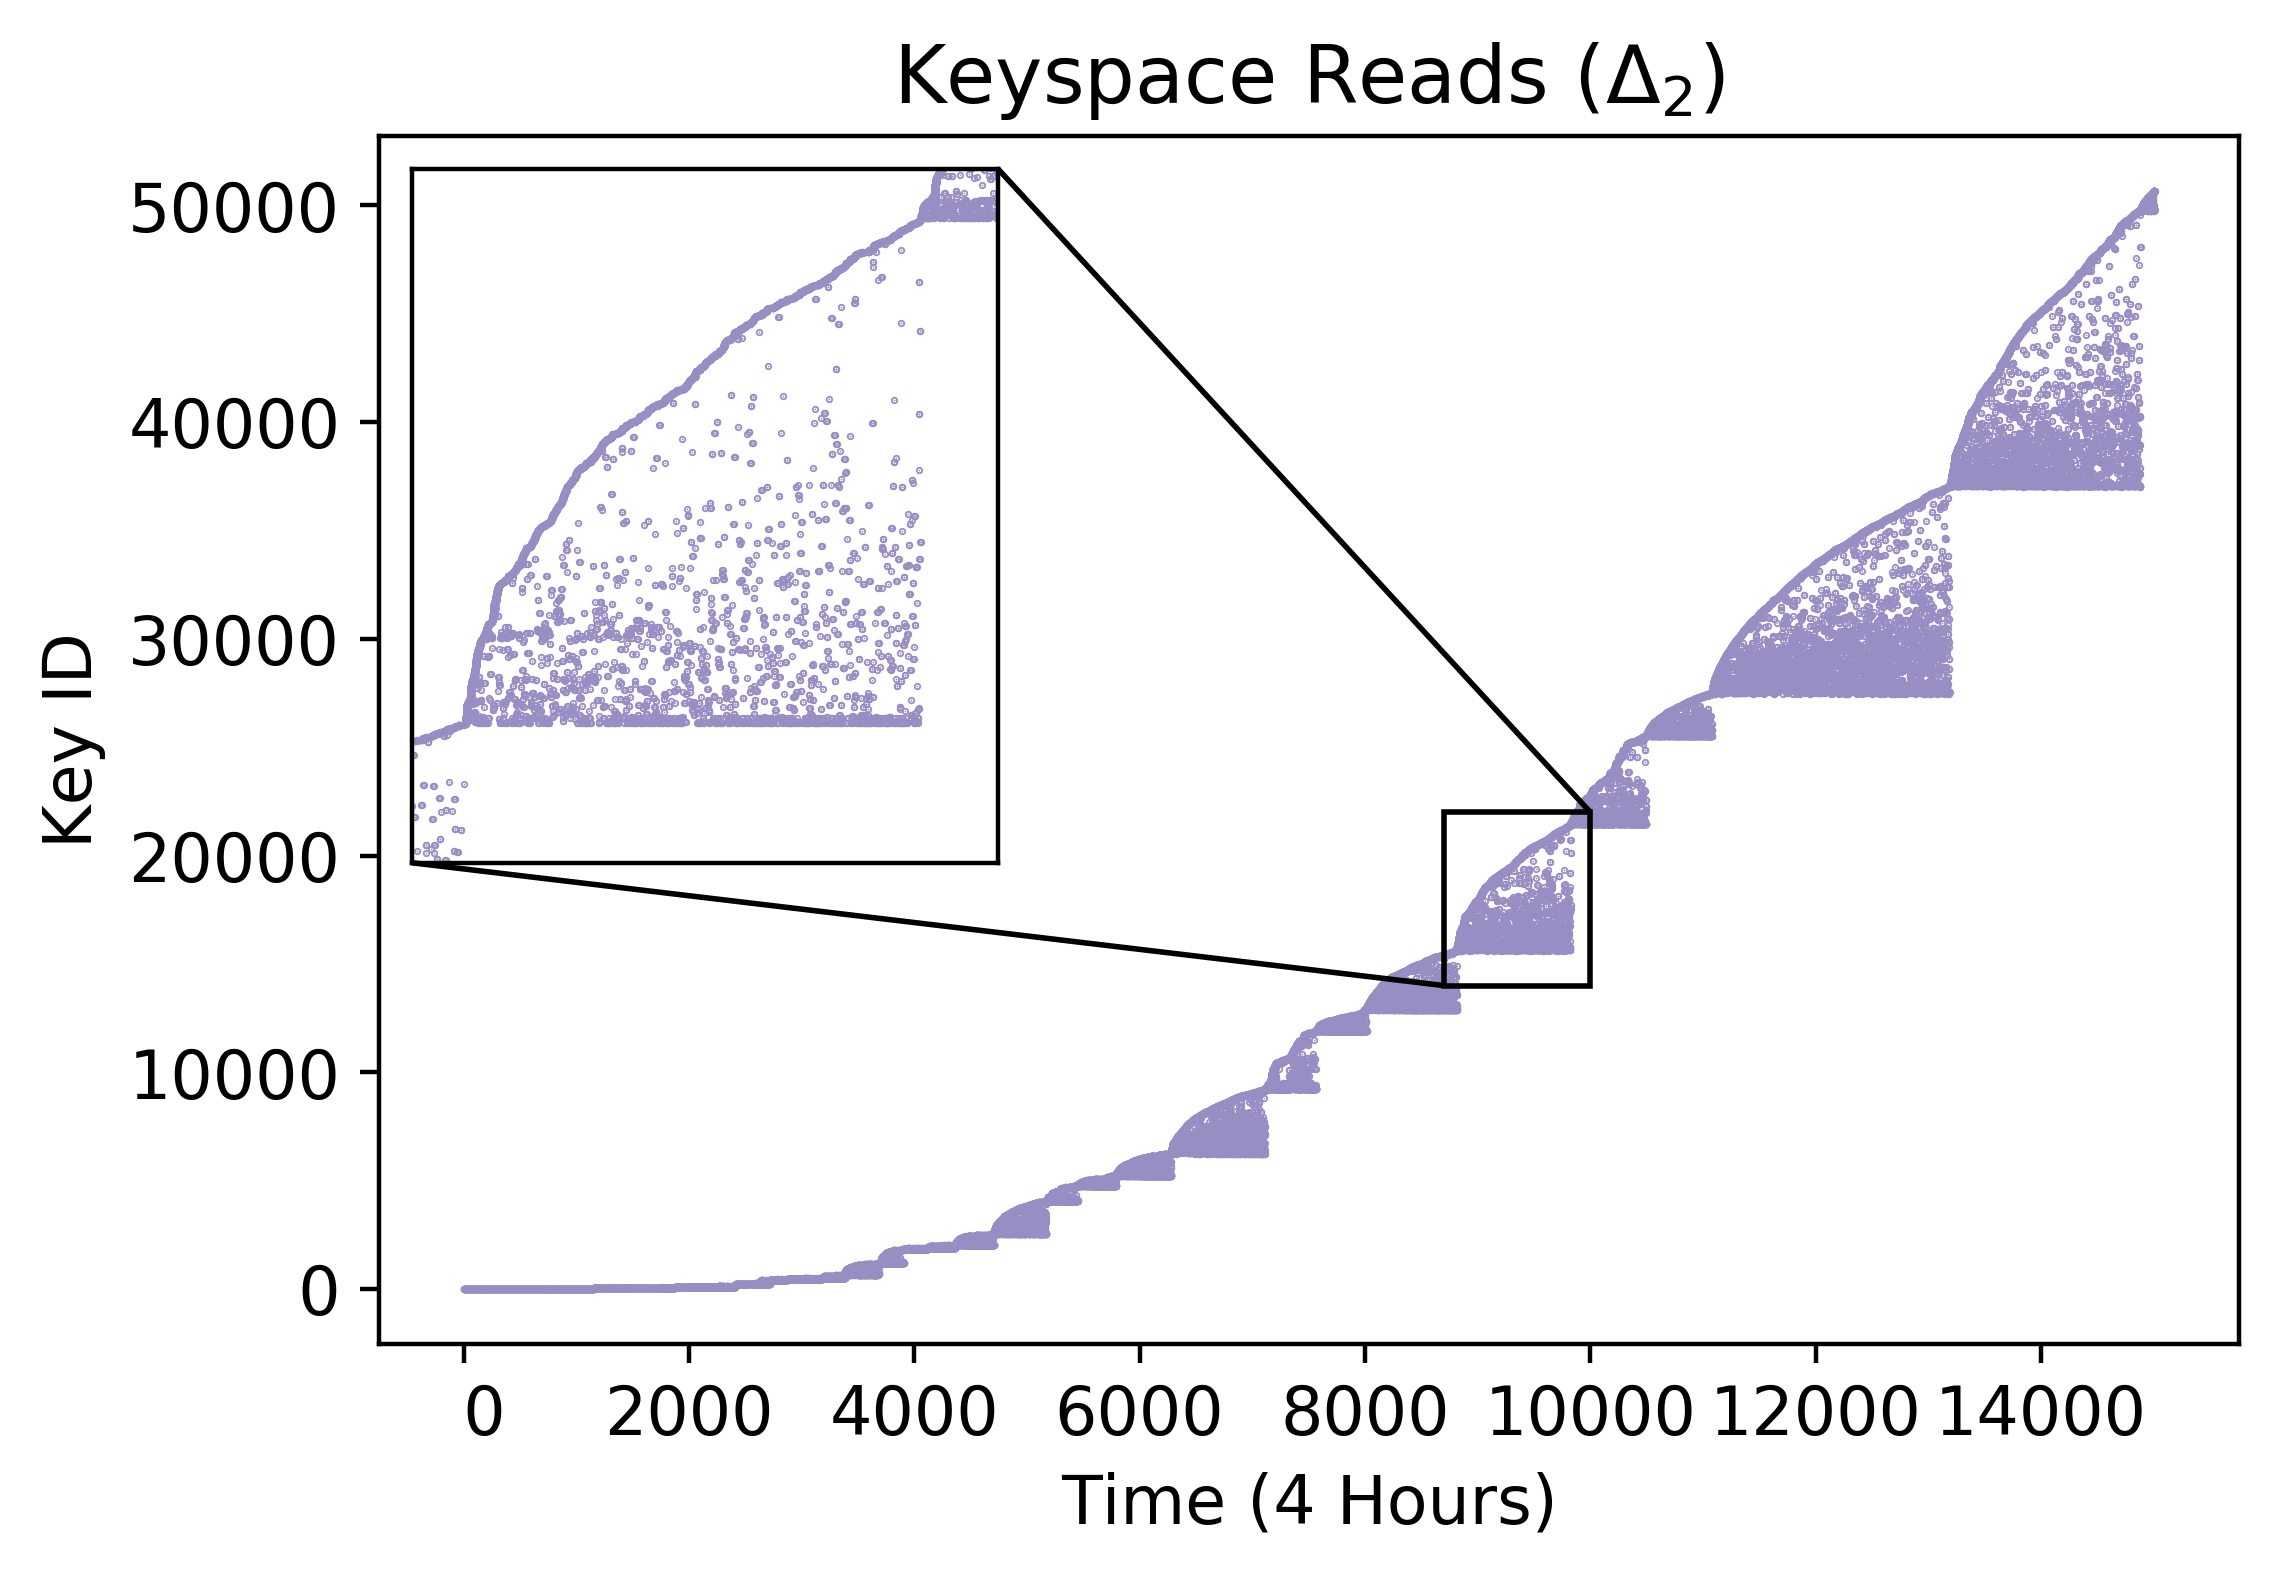
\includegraphics[height=5cm,width=0.4\textwidth]{figures/keyspace-zoomed.png}\\
%
%  \caption{Key activity for a 4 hour run shows groups of accesses to the same
%  subset of keys. Detecting these access patterns leads to a more accurate cache
%  management strategy.\label{fig:keyspace-zoomed}}
%
%\end{figure}
%
%\begin{figure}[t]
%\noindent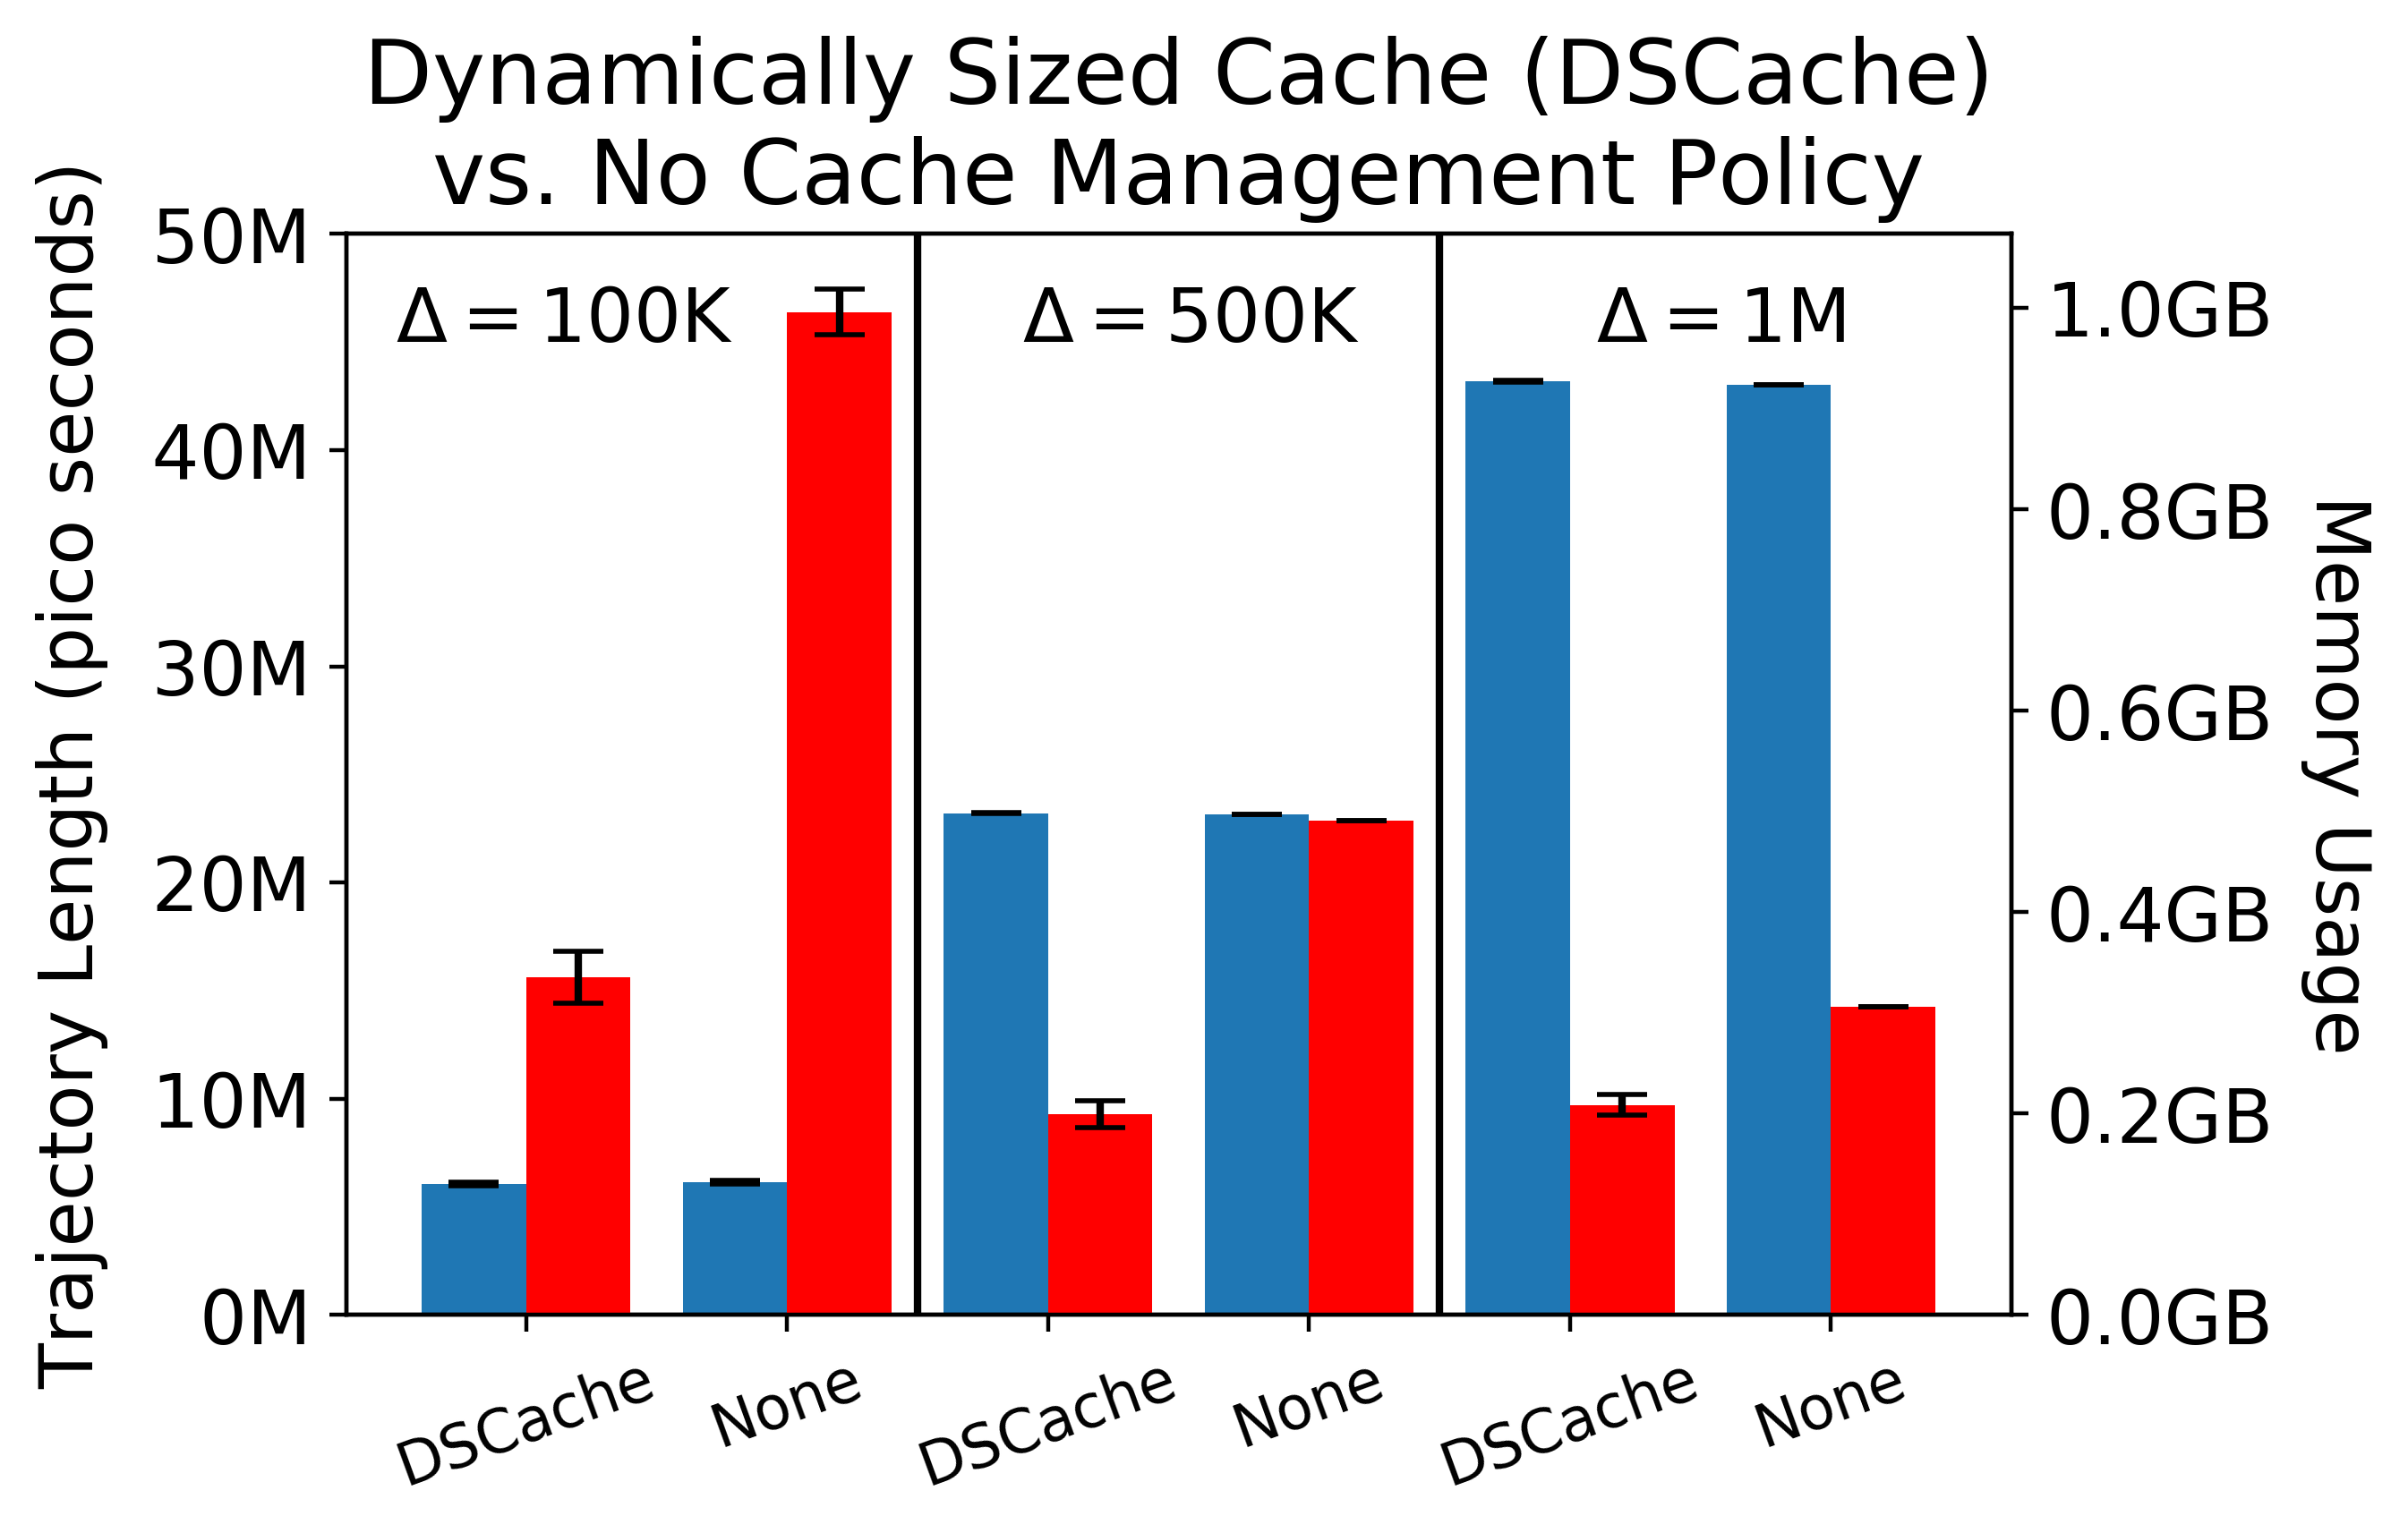
\includegraphics[width=0.5\textwidth]{figures/dscache-vs-none.png}\\
%
%\caption{The performance and resource utilization trade-off for the dynamically
%sized cache (DSCache) policy compared to no cache management. With a negligible
%performance impact, DSCache adjusts to different initial conditions
%(\(\Delta\)) automatically and saves over 2\(\times\) memory in the best case.
%\label{fig:dscache-vs-none}}
%\end{figure}
%
%\begin{figure}[t]
%\noindent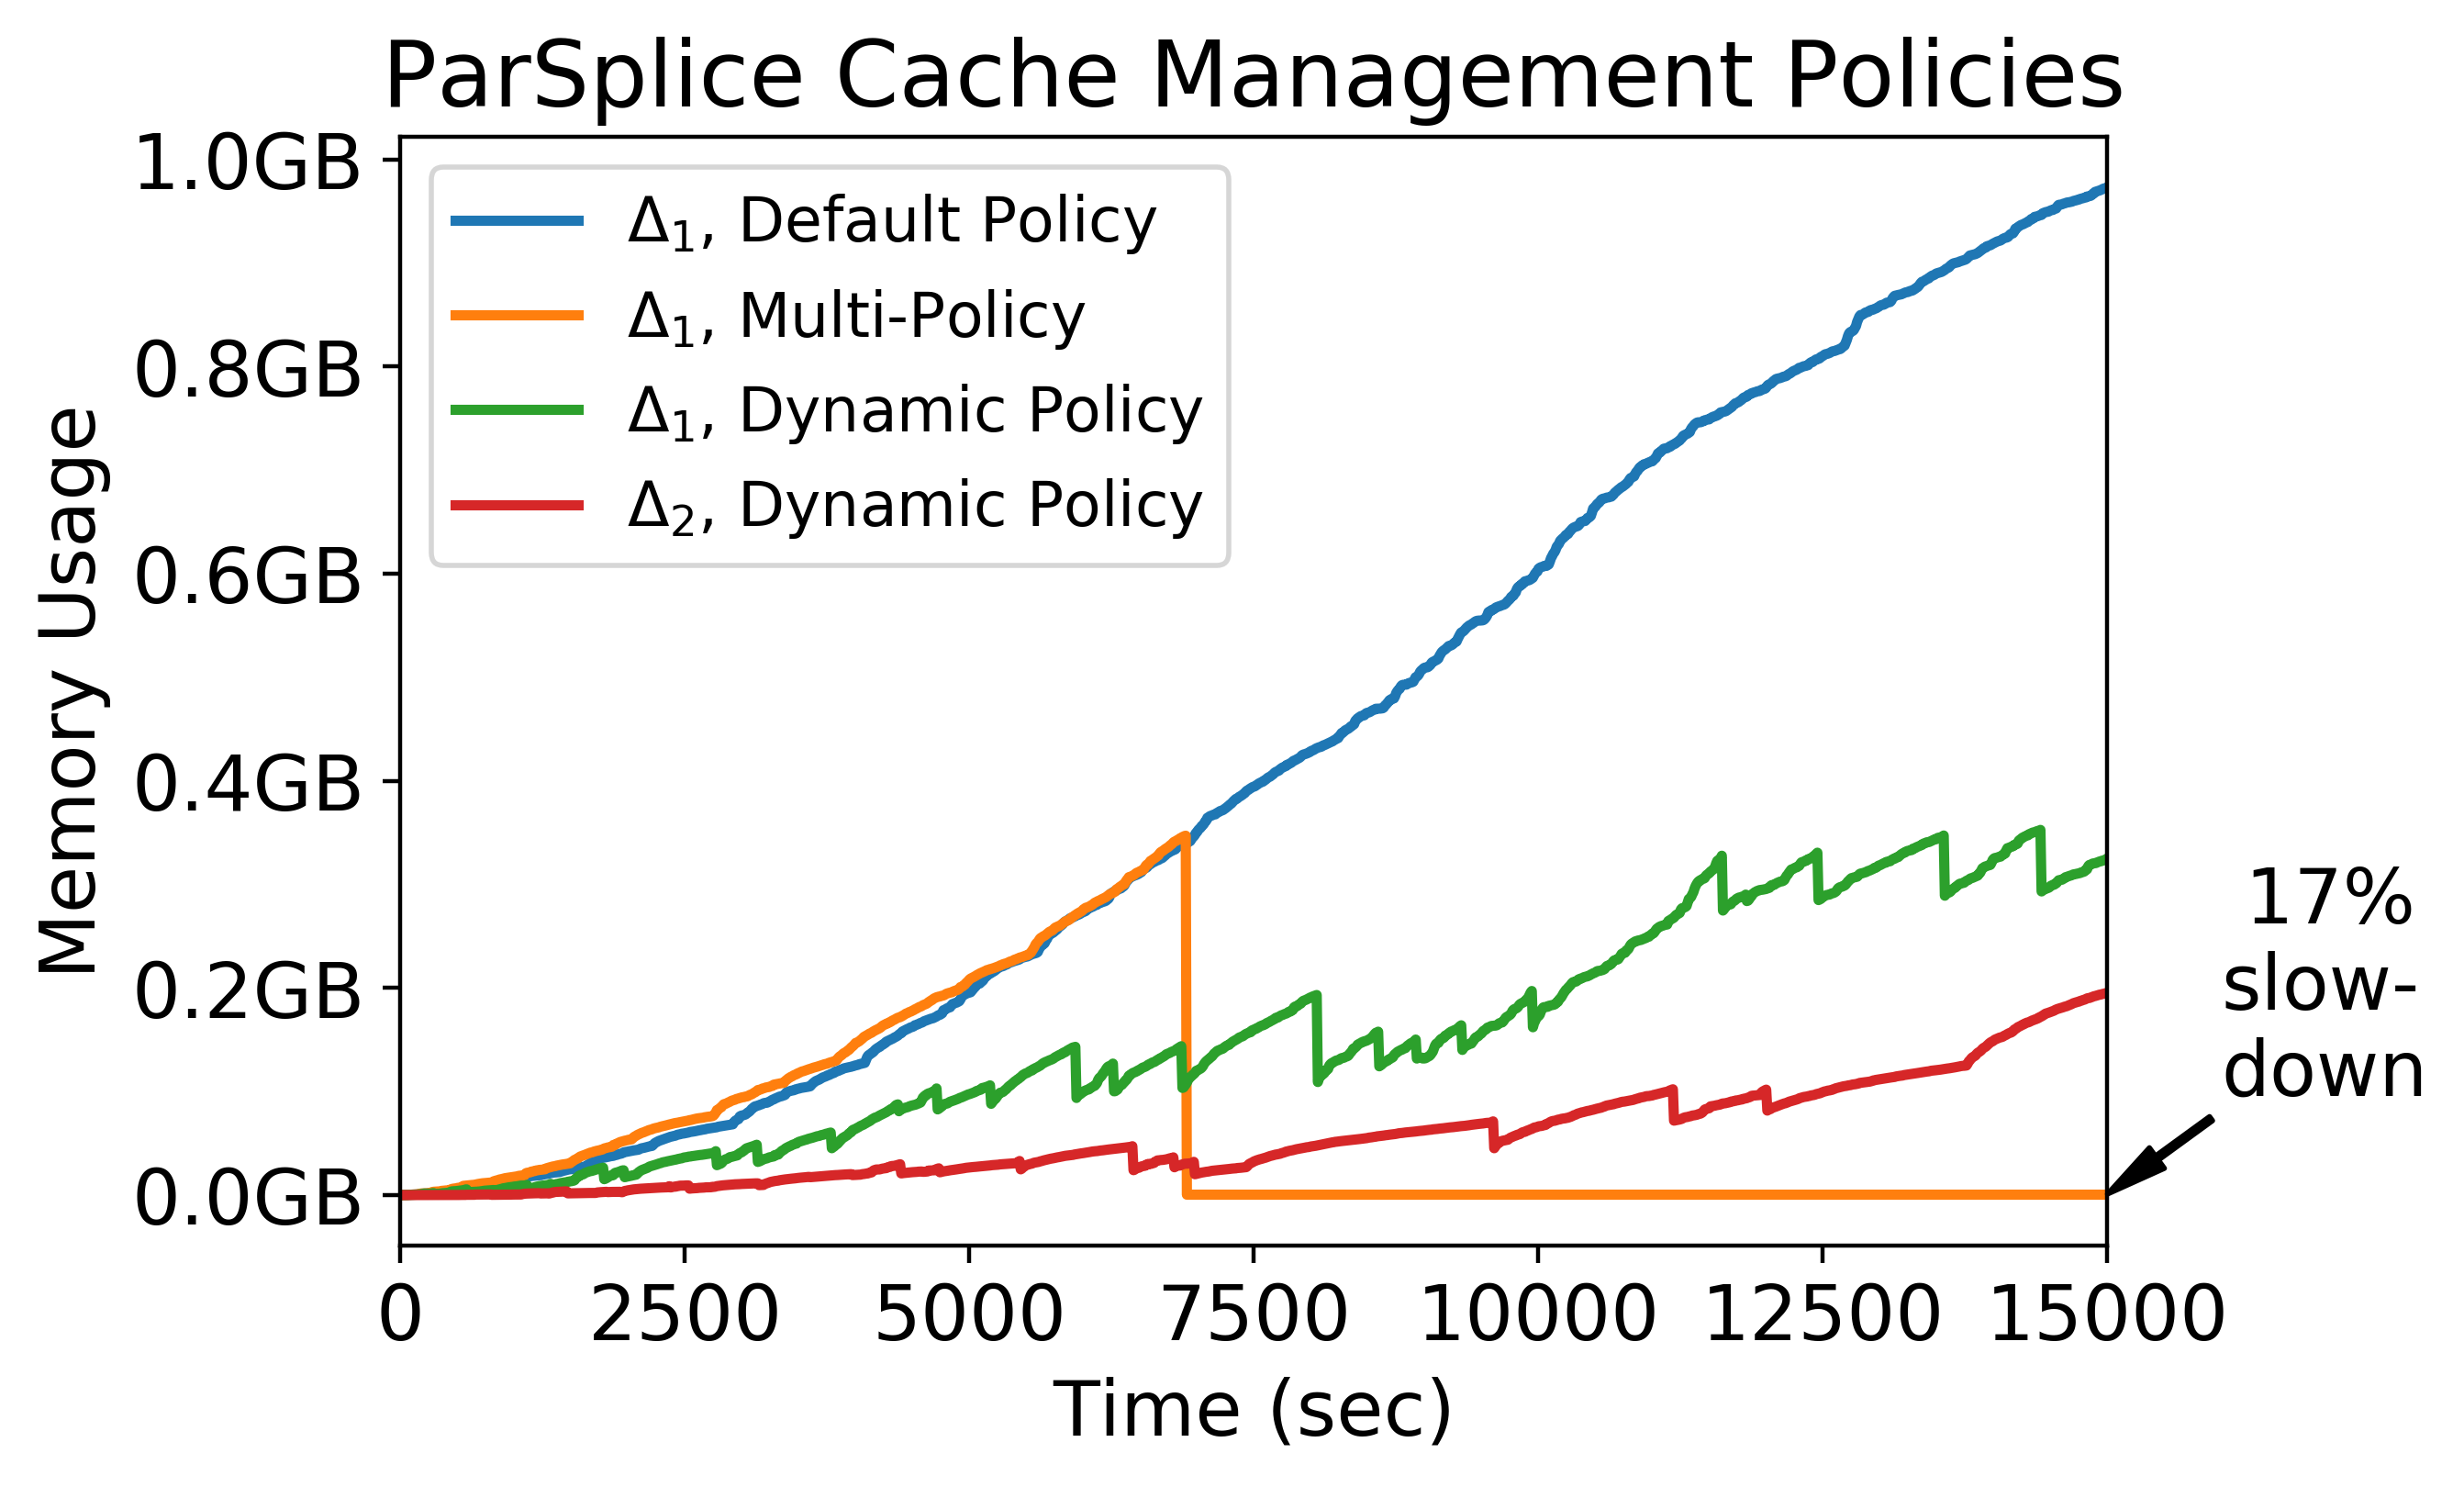
\includegraphics[width=0.5\textwidth]{figures/memory-vs-time.png}\\
%
%\caption{Memory utilization of different cache management policies.  ``No Cache
%Management" allows unlimited cache growth, ``Multi-Policy" absorbs the initial
%burstiness of the workload before switching to a more constrained cache, and
%the ``Dynamic Policy" curves size the cache according to key access patterns.
%We show a \(\Delta_2\) growth rate to demonstrate the dynamic policy's ability
%to adjust to a different set of initial conditions.\label{fig:memory-vs-time}}
%\end{figure}

Feeding application-specific knowledge about ParSplice into a policy
leads to a more accurate cache management strategy.  The goal of the following
section is not to find an optimal solution, as this can be done with parameter
sweeps for thresholds; rather, we try to find techniques that work for a range
of inputs and system setups.

Figure~\ref{fig:keyspace-zoomed} shows which keys (\(y\) axis) are accessed by
tasks over time (\(x\) axis). The groups of accesses to a subset of keys occurs
because the system is stuck in so-called superbasins, {\it i.e.} coarse regions of space from
which it is difficult to escape, but within which it is easy to move. Systems
stuck in superbasins will explore the same set of minima for a
long time, leading to the same keys being accessed repeatedly. In
Figure~\ref{fig:keyspace-zoomed}, superbasins are typically not re-visited because the
simulation only adds atoms; we can never revisit a superbasin that contains less atoms
than the simulation currently contains.
This is why keys are never re-accessed after a given amount of time.

Detecting these superbasins can lead to more effective cache management
strategies because the height of the groups of key accesses is ``how much" of
the cache to evict and the width of the groups of key accesses is ``when" to
evict values from the cache.  The zoomed portion of
Figure~\ref{fig:keyspace-zoomed} shows how a single superbasin affects the key
accesses. Moving along the \(x\) axis shows that the number of unique keys
accessed over time grows while moving along the \(y\) axis shows that early
keys are accessed more often.  Despite these patterns, the following
characteristics of superbasins make them hard to detect:

\begin{itemize}

  \item superbasin key accesses are random and there is no threshold ``minimum distance
  between key access" that indicates we have moved on to a new superbasin

  \item superbasins change immediately

  \item the number of keys a superbasin accesses differs from other superbasins

\end{itemize}

\subsection{Failed Strategies}

To detect the access patterns in Figure~\ref{fig:keyspace-zoomed}, we try a
variety of techniques using Mantle. Unfortunately, we found that the following
techniques proliferate more parameters that need to be tuned per
hardware/software configuration. Furthermore, many of the metrics do not signal
a new set of key accesses.  Below, we indicate with quotes which parameters we
need to add for each technique and the value we find to work best, via
tuning and parameter sweeps, for one set of initial conditions.

\begin{itemize}

  \item Statistics: decay on each key counts down until 0; 0-valued keys are
evicted.  ``history-of-key-accesses", set to 10 seconds, to evict keys.

  \item Calculus: use derivative to strip away magnitudes; use large positive
slopes followed by large negative slope as signal for new set of key accesses.
``Zero-crossing", set to 40 seconds, for distance between small/large spikes to
avoid false positives; ``window size", set to 200 seconds, for the size of the
moving average.

  \item K-Means Clustering fails because ``K" is not known {\it a-priori} and
groups of key accesses are different size. ``K", set to 4, for the number of clusters in the data
using the sum of the distances to the centroid.

  \item DBScan: finds clusters using density as a metric. ``Eps", set to 20, for
max distance between 2 samples in same neighborhood; ``Min", set to 5, for the
samples per core.

  \item Edge Detection: size of the image is too big and bottom edges are
not thick enough.

\end{itemize}

\subsection{Dynamically Sized Cache: Access Pattern Detection}
\label{sec:regime-detection}

After trying these techniques we found that the basic O(\(n\)) algorithm in
Figure~\ref{src:dyn-cache} works best. The algorithm detects groups of key
accesses, which we call ``fans", by iterating backwards through the key access
trace, finding the lowest key ID, and comparing against the lowest key ID we
have seen so far (Line 7). We also maintain the top and bottom of each group of
key accesses (Line 13) so we can tell the ``how much" policy the number of keys
to evict (Line 23).  The algorithm is O(\(n\)), where \(n\) is the number
events, but the benefit is that the approach avoids adding new thresholds for
key access pattern detection ({\it e.g.}, space between key accesses, space
between key IDs, and window size of consecutive key accesses).

The algorithm iterates backwards over the key access trace because a change in
the minimum value signals a new group of key accesses. No signal exists
iterating left to right, as the maximum value always increases and the minimum
values at the bottom of each group of key accesses are sparse.  For example,
the maximum distance between values along the bottom edge of the zoomed group
of key accesses in Figure~\ref{fig:keyspace-zoomed} is 125 seconds, while the
maximum distance between minimum values for the group of key accesses before is
0 seconds. As a result of this sparseness, iterating left to right requires a
``window size" parameter to determine when we think a minimum value will not
show up again.  

The performance and memory utilization is shown by the ``DSCache" bars in
Figure~\ref{fig:dscache-vs-none}. Without sacrificing performance (trajectory
length), the dynamically sized cache policy uses between 32\%-66\% less memory
than the default ParSplice configuration (no cache management) for the 3
initial conditions we test. The memory usage over time is shown by the ``Dynamic Policy"
curves in Figure~\ref{fig:memory-vs-time}, where the behavior resembles the key
access patterns in Figure~\ref{fig:keyspace-zoomed}\footnote{The memory usage
is not {\it exactly} the same because these are two different runs;
Figure~\ref{fig:keyspace-zoomed} has key activity tracing turned on, which
reduces performance.}.  We also show a \(\Delta_2\) growth rate to demonstrate
the dynamic policy's ability to adjust to a different set of initial
conditions.



\section{Towards General Data Management Policies}
\label{sec:scope}

\begin{figure*}[t!]
    \centering
    \begin{subfigure}[t]{0.48\textwidth}
        \centering
        \footnotesize
        \centering
        \begin{minted}[xleftmargin=3em,linenos]{lua}
function when()
  if server[whoami]['cachesize'] > n then
    if server[whoami]['cachesize'] > 100K then
      WRstate(1)
    end
    if RDstate() == 1 then
      return true
    end
  end
  return false
end
        \end{minted}
        \caption{ParSplice cache management policy that absorbs the burstiness of the
        workload before switching to a constrained cache.  The
        performance/utilization for different  \texttt{n} is in
        Figure~\ref{fig:methodology-tradeoff}. \label{src:lru-dyn}}
    \end{subfigure}%
    ~ 
    \begin{subfigure}[t]{0.48\textwidth}
        \centering
        \footnotesize
        \begin{minted}[xleftmargin=3em,linenos]{lua}
local function when()
  if servers[whoami]["load"] > target then
    overloaded = RDstate() + 1
    WRstate(overloaded)
    if overloaded > 2 then
      return true
    end
  end
  else then WRstate(0) end
  return false
end
        \end{minted}
	\caption{CephFS file system metadata load balancer, designed in 2004
        in~\cite{weil:sc2004-dyn-metadata}, reimplemented in Lua
        in~\cite{sevilla:sc15-mantle}. This policy has many similarities to the
        ParSplice cache management policy.\label{src:lua-cephfs}}
    \end{subfigure}
    \caption{ParSplice's cache management policy has the same components as
    CephFS's load balancing policy.}
\end{figure*}



%\begin{itemize}
%  \item Lustre Trace
%  \item LinkedIn Trace
%  \item Nathan's Trace
%\end{itemize}

In the previous section, we used our data management language and the Mantle
policy engine to design effective cache management strategies for a new
application and storage system. In this section, we compare and contrast the
policies examined for file system metadata load balancing
in~\cite{sevilla:sc15-mantle} with the ones we designed and evaluated above for
cache management in ParSplice. 

\subsection{Using Load Balancing Policies for Cache Management}

%- memory utilization/heuristics
From a high-level the cache management policy we designed in
Figure~\ref{src:lru-dyn} trims the cache if the cache reaches a certain size
{\it and} if it has already absorbed the initial burstiness of the workload.
Much of this implementation was inspired by the CephFS metadata load
balancing policy in Figure~\ref{src:lua-cephfs}, which was presented
in~\cite{sevilla:sc15-mantle}. That policy migrates file system metadata if the
load is higher than the average load in the cluster {\it and} the current
server has been overloaded for more than two iterations. The two policies have
the following in common:

\textbf{Condition for ``Overloaded"} (Fig.~\ref{src:lru-dyn}: Line 2;
Fig.~\ref{src:lua-cephfs}: Line 2) - these lines detect whether the node is
overloaded using the load calculated in the load callback (not shown). While
the calculations and thresholds are different, the way the loads are used is
exactly the same; the ParSplice policy flags the node as overloaded if the
cache reaches a certain size while the CephFS policy compares the load to other
nodes in the system.

\textbf{State Persisted Across Decisions} (Fig.~\ref{src:lru-dyn}: Lines 4,6;
Fig~\ref{src:lua-cephfs}: Lines 3,4,9) - these lines use Mantle to write/read state
from previous decisions.  For ParSplice, we save a boolean that indicates
whether we have absorbed the workload's initial burstiness. For CephFS, we save
the number of consecutive instances that the server has been overloaded. We
also clear the count (Line 9) if the server is no longer overloaded. 

\textbf{Multi-Policy Strategy} (Fig.~\ref{src:lru-dyn}: Line 6;
Fig.~\ref{src:lua-cephfs}: Line 5) - after determining that the node is
overloaded, these lines add an additional condition before the policy enters a
data management state.  ParSplice trims its cache once it eclipses the
``absorb" threshold while CephFS allows balancing when overloaded for more than
two iterations. The persistent state is essential for both of these
policy-switching conditions.

These similarities among effective policies for two very different domains
suggest that the heuristics and techniques in other load balancers can be used
for cache management. The result support the notion that concepts and problems
that architects grapple with are transcendent and the solutions they design can
be re-used in different code bases.

\subsection{Using Cache Management Policies for Load Balancing}

\begin{figure}[t]
\noindent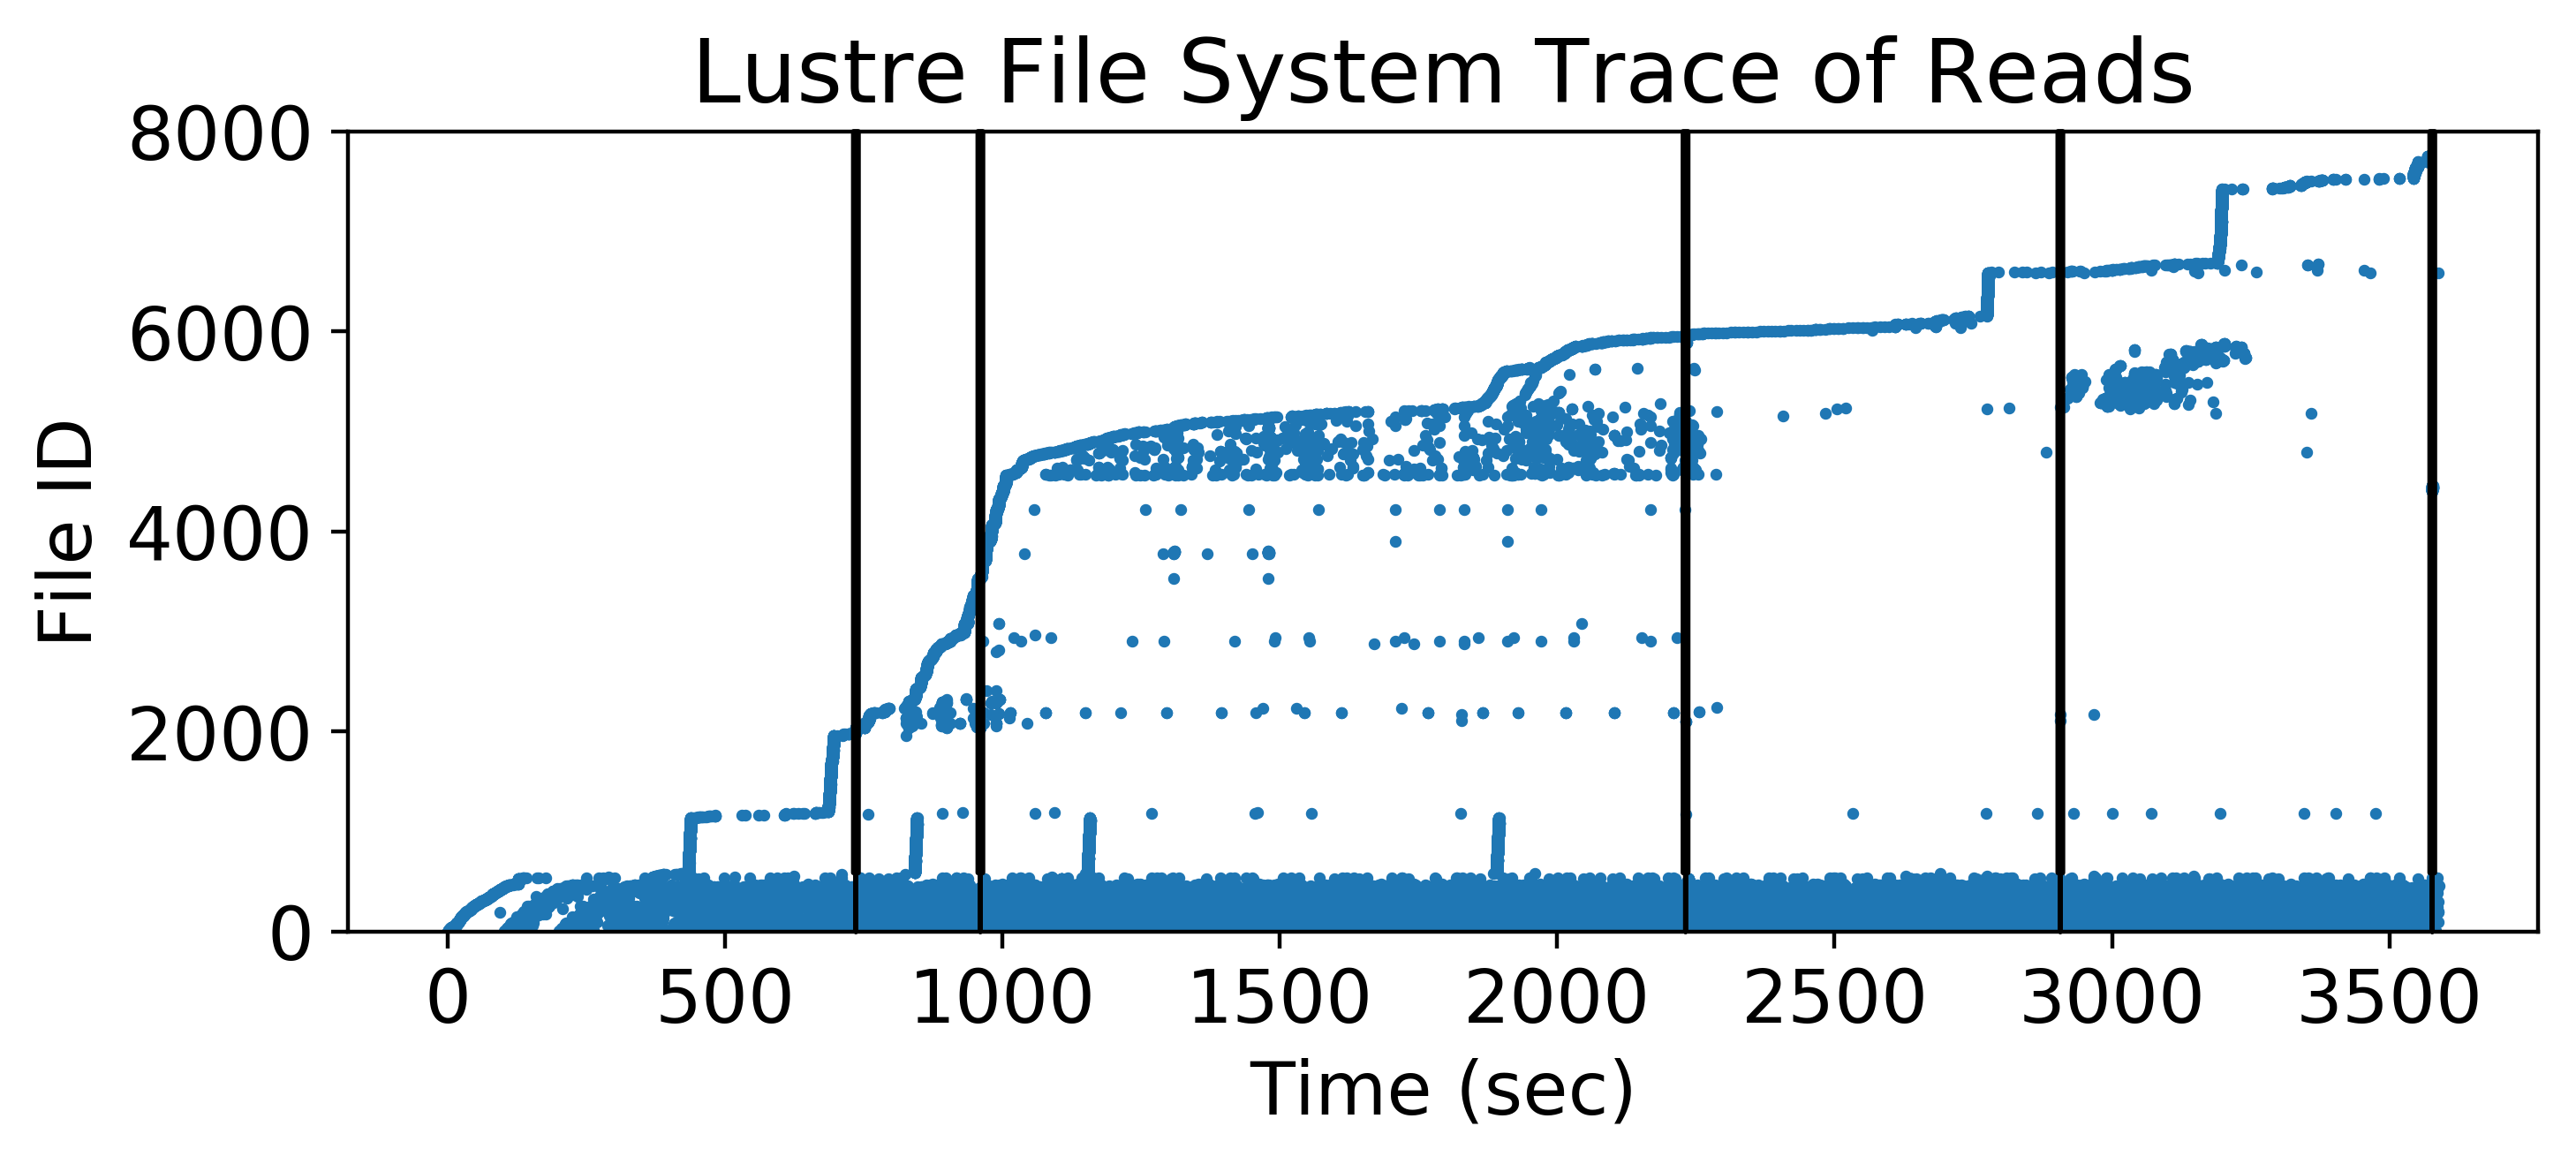
\includegraphics[width=0.5\textwidth]{figures/trace-atime.png}\\
\caption{File system metadata reads for a Lustre trace collected at LANL. The
vertical lines are the access patterns detected by the ParSplice cache
management policy from Section~\S\ref{sec:dom-specific}. The policy works
``out-of-the-box", which suggests that data management policies are general and
can be used across domains.
\label{fig:trace-atime}}
\end{figure}

%- how many inodes to keep in mds/client caches
%- affects LB; increases capacity of single MDS (reduces req/mem pressure)
%- affects LB; tells us which part of the cache to keep local

The cache management policies we developed earlier can be used by load
balancing policies to effectively spread load across a cluster. For example,
distributed file systems that load balance file system metadata across a
dedicated metadata cluster could use the caching policies to determine what
metadata to move and when to move it.  To demonstrate this idea, we analyze a
3-day Lustre file system metadata trace, collected at LANL.  The trace is
anonymized so all file names are replaced with a unique identifier and we do
not know which applications are running. We visualize a 1 hour window of the
trace in Figure~\ref{fig:trace-atime}, where the dots are the file system
metadata reads in a 1 hour window.  The \(x\) axis is time and the \(y\) axis
is the file ID, listed in the order that file IDs appear in the trace.  The
groups of accesses look similar to the ParSplice key accesses in
Figure~\ref{fig:keyspace-zoomed}. 

Although other access pattern detection algorithms are possible, we use the one
designed for cache management in Section~\S\ref{sec:regime-detection} with
slight modifications based on our knowledge of file systems\footnote{We
filtered out requests for key IDs less than 2000, as these are most likely path
traversal requests to higher parts of the namespace.}. The vertical lines in
Figure~\ref{fig:trace-atime} are the groups of accesses identified by the
algorithm; it successfully detects the largest group of key accesses that
starts at time 1000 seconds and ends at time 2200 seconds. File systems that
load balance file system metadata across a cluster would want to keep metadata
in that group of key accesses on the same server for locality and would want to
avoid migrating metadata to a different server until the group of key accesses
completes.

Before we showed how policies designed for load balancing heavily influence our
cache management in a different application and storage system. But in this
section we show how an {\it unmodified} cache management policy can be used in
a load balancing strategy.  This generalization may reduce the work that needs to
be done for load balancing as ideas may have already been explored in other
domains and could work ``out-of-the-box". 

%% burstiness of creates then compile
%Cache management can also increase the capacity of a single server, which
%affects how load should be distributed across a cluster.  For example, CephFS
%clients and servers maintain a consistent cache so that the client can do
%operations locally without contacting the metadata server.  But large caches
%use more memory, so having smart policies that detect key access patterns would
%greatly reduce memory footprints. For example, Figure~\ref{fig:compile-ops}
%shows the trace of metadata requests for compiling code in CephFS.  The \(y\)
%axis is  the number of file system metadata requests serviced by the metadata
%server when uncompressing (\texttt{untar}), compiling (\texttt{make}), and
%deleting (\texttt{rm}) the source code for the Linux kernel. If the system
%knows that the job phases would progress from many creates, to many lookups, to
%many deletes, then it could size its caches accordingly. For example, the file
%system could cache none of the metadata from the \texttt{untar} phase and run
%key access pattern detection during the \texttt{make} phase, resulting in the
%metadata server/clients only caching metadata that is repeatedly used. For the
%job in Figure~\ref{fig:compile-ops}, this would fill up the cache to only 20K
%inodes (the unit of metadata for file systems) instead of 60K, resulting in
%almost 40MB of memory savings (since an inode is about
%1KB\footnote{http://docs.ceph.com/docs/master/dev/mds\_internals/data-structures/})
%without sacrificing performance.
%
%%- strategy: cache all inodes on create
%\begin{figure}[t]
%\noindent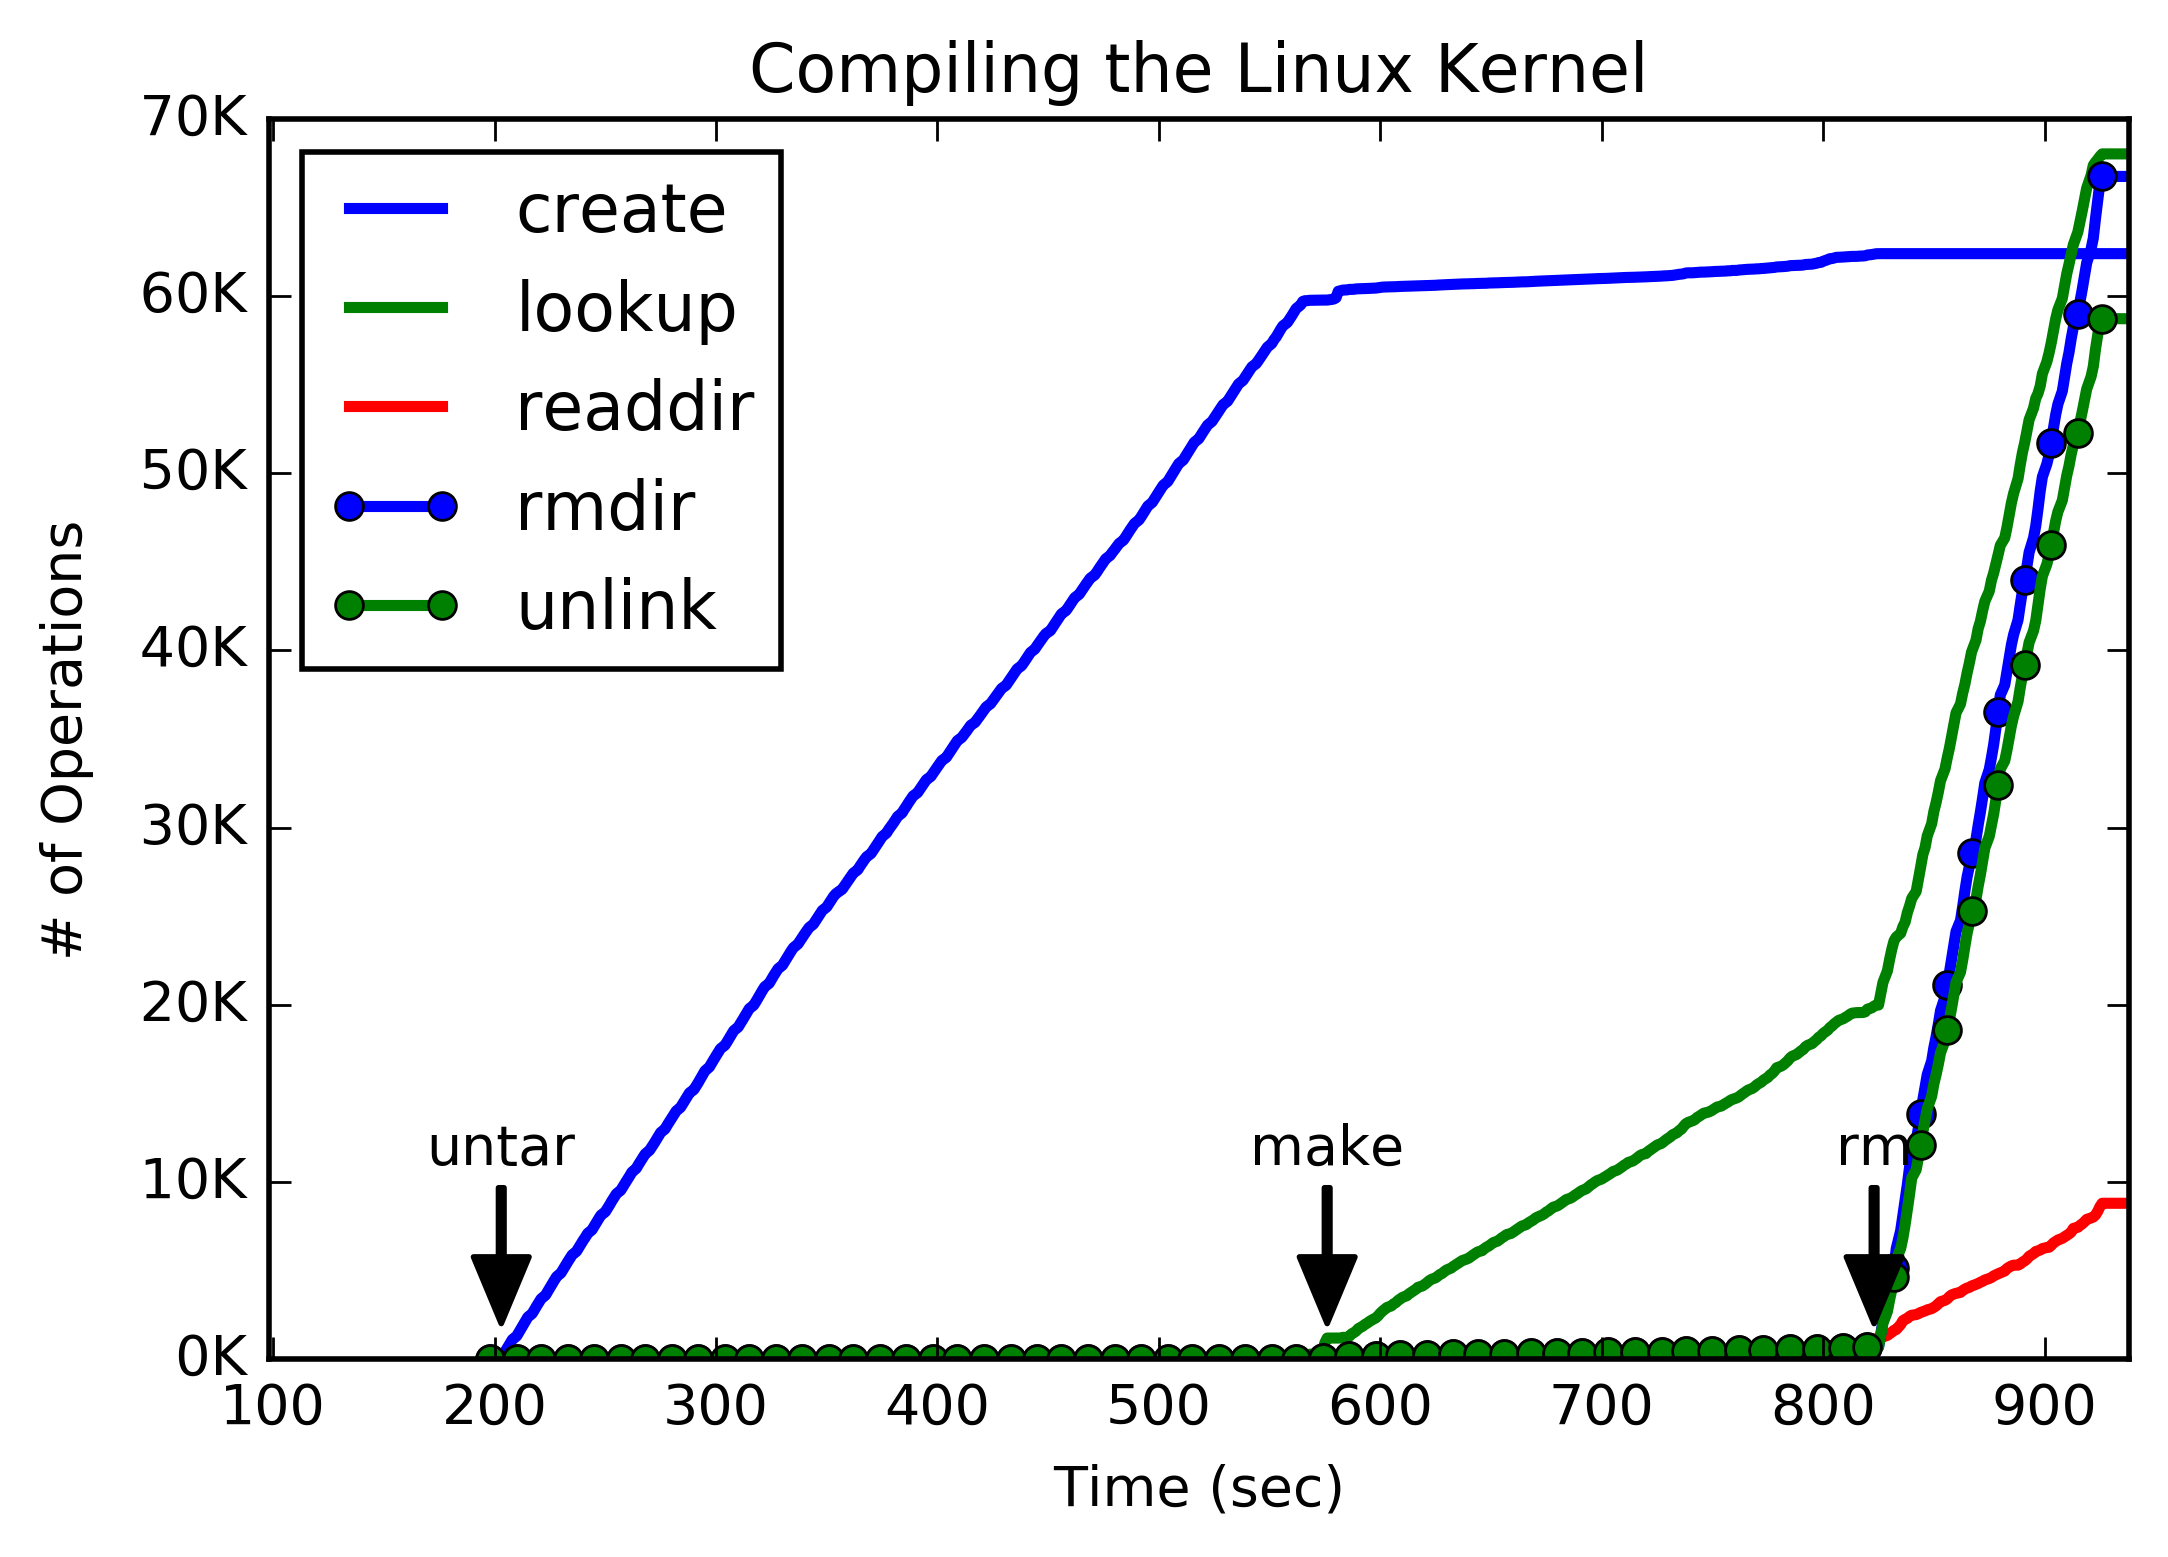
\includegraphics[width=0.5\textwidth]{figures/compile-ops.png}\\
%\caption{File system metadata requests for a compile job show workload phases
%characterized by a dominant request type ({\it e.g.}, creates for ``untar").
%Using ParSplice cache management policies for these types of workloads would
%reduce memory pressure without sacrificing performance.
%\label{fig:compile-ops}}
%\end{figure}

\subsection{Other Use Cases}

% other use cases caches/tiers 
Storage systems have many other data management techniques that would benefit
from the caching policies developed in Sections~\S\ref{sec:arch-specific}
and~\ref{sec:dom-specific}. For example, Ceph administrators can use the
policies in ParSplice to automatically size and manage cache
tiers\footnote{http://docs.ceph.com/docs/master/rados/operations/cache-tiering/},
caching on object storage devices, or in the distributed block
devices\footnote{http://docs.ceph.com/docs/master/rbd/rbd-config-ref/}.
Integration with Mantle would be straightforward as it is merged into Ceph's
mainline\footnote{http://docs.ceph.com/docs/master/cephfs/mantle/} and the
three caching subsystems mentioned above already maintain key access traces. 

More generally, the similarities between load balancing and cache management
show how the ``when"/``where"/``how much" abstractions, data management
language, and policy engine may be widely applicable to other data management
techniques, such as:

\begin{itemize}

  \item QoS: when to move clients, where to move clients, how much of the
reservation to move. We could use Mantle to implement something like the
reservation algorithms based on utilization and period in
Fahrrad~\cite{povzner_horizon_2010} to achieve better guarantees without
sacrificing performance.

  \item Scheduling: when to yield computation cycles to another process, how
much of a resource to allocate. We could use Mantle to implement the
fairness/priority models used in the Mesos~\cite{hindman_mesos_2011} ``how
many" policies.

  \item Batching: how many operations to group together, when to send large
batches of updates. We could use Mantle to implement pathname leases from
IndexFS~\cite{ren:sc2014-indexfs} or the capabilities from
CephFS\footnote{http://docs.ceph.com/docs/master/cephfs/capabilities/}.

  \item Prefetching: how much to prefetch, how to select data.  We could use
Mantle to implement forward/backward/stride detection algorithms for
prefetching in RAID arrays or something more complicated, like the time series
algorithms for adaptive I/O prefetching from~\cite{tran:sc01-arima}.

\end{itemize}

\section{Related Work}

Key-value storage organizations for scientific applications is a field gaining
rapid interest. In particular, the analysis of the ParSplice keyspace and the
development of an appropriate scheme for load balancing is a direct response to
a case study for computation caching in scientific
applications~\cite{jenkins:ipdsw17-mochi}. In that work the authors motivated
the need for a flexible load balancing \emph{microservice} to efficiently scale
a memoization microservice. Our work is also heavily influenced by the
Malacology project~\cite{sevilla:eurosys17-malacology} which seeks to provide
fundamental services from within the storage system ({\it e.g.}, consensus) to
the application.

State-of-the-art distributed file systems partition write-heavy workloads and
replicate read-heavy workloads, similar to the approach we are advocating
here.  IndexFS~\cite{ren:sc2014-indexfs} partitions directories and clients
write to different partitions by grabbing leases and caching ancestor metadata
for path traversal. ShardFS takes the replication approach to the extreme by
copying all directory state to all nodes. The Ceph file system
(CephFS)~\cite{weil:sc2004-dyn-metadata, weil:osdi2006-ceph} employs both
techniques to a lesser extent; directories can be replicated or sharded but the
caching and replication policies are controlled with tunable parameters.  These
systems still need to be tuned by hand with {\it ad-hoc} policies designed for
specific applications.  Setting policies for migrations is arguably more
difficult than adding the migration mechanisms themselves.  For example,
IndexFS/CephFS use the GIGA+~\cite{patil:fast2011-giga} technique for
partitioning directories at a \emph{predefined} threshold. Mantle makes headway
in this space by providing a framework for exploring these policies, but does
not attempt anything more sophisticated (e.g., machine learning) to create
these policies. 

% ml and autotuning
Auto-tuning is a well-known technique used in
HPC~\cite{behzad:sc2013-autotuning, behzad:techreport2014-io-autotuning}, big
data systems systems~\cite{herodotou_starfish_2011}, and
databases~\cite{schnaitter_index_2009}.  Like our work, these systems focus on
the physical design of the storage ({\it e.g.} cache size) but since we focused
on a relatively small set of parameters (cache size, migration thresholds), we
did not need anything as sophisticated as the genetic algorithm used
in~\cite{behzad:sc2013-autotuning}.  We cannot drop these techniques into
ParSplice because the magnitude and speed of the workload hotspots/flash crowds
makes existing approaches less applicable. 

Our plan is to use MDHIM~\cite{greenberg:hotstorage2015-mdhim} as our back-end
key-value store because it was designed for HPC and has the proper mechanisms
for migration already implemented.  

\section{Future Work}

This lays the foundation for future work, where we will focus on formalizing a
collection of general data management policies that can be used across domains
and services. The value of such a collection eases the burden of policy
development and paves the way for solutions that remove the administrator from
the development cycle, such as (1) adaptable policies that automatically switch
to new strategies when the current strategy behaves poorly ({e.g.}, thrashing,
making no progress, etc.), and (2) policy generation, where new policies are
constructed automatically by examining the collection of existing policies.
Such work is made possible with Mantle's ability to dynamically change
policies.

\section{Conclusion}

Data management encompasses a wide range of techniques that vary by domain and
service. Yet, the techniques require policies that shape the decision making
and finding the best policies is a difficult, multi-dimensional problem. We
observe that many of the primitives and resulting strategies have enough in
common that they can be expressed with similar semantics. We present a data
management language and policy engine, called Mantle that is general enough to
express complicated, dynamic policies for two different domains and services.
Rather than attempting to construct a single, complex load balancing policy
that works for a variety of scenarios, we instead use the Mantle framework to
enable software-defined storage systems to flexibly change policies as the
workload changes over time.  In our analysis of the ParSplice key-value
workload we have detected clear workload regimes that are sensitive to the
initial conditions and the scale and duration of the simulation. We have also
demonstrated that changing load balancing policies at runtime in response to
the current workload is an effective mechanism to providing better load
distribution.  Finally, we have demonstrated that Mantle is flexible enough to
support domain-specific knowledge, which lays the groundwork for future work in
adaptable policies and policy generation.



\bibliographystyle{IEEEtran}
\bibliography{IEEEabrv,paper}

\end{document}
